\documentclass{article}
\usepackage{float}
\usepackage{amsmath}
\usepackage{amssymb}
\usepackage{tikz}
\usetikzlibrary{shapes.geometric}
\usepackage{pgfplots}
\pgfplotsset{compat=1.18}
\usepackage{hyperref}
\hypersetup{
    colorlinks=true,
    linkcolor=black,
    filecolor=magenta,      
    urlcolor=cyan,
}

\title{Multimedia information retrieval and computer vision\\
\large Lecture notes}
\author{Ettore Ricci}

\begin{document}
\maketitle
\tableofcontents

\section{Information retrieval}
\subsection{Basic Retrieval}
\label{sec:basic_retrieval}

An IR system resembles and has evolved from a library.
Now they are Google, DuckDuckGo, Bing, etc.
Whenever we have a "search bar" we are using an IR system.
Also image, audio, legal and medical retrieval systems exist.

Imagine searching for a word in a book, it would be
slow enough with $O(100)$ pages, imagine with $O(1B)$ pages.
Linear search is not feasible, that's why we need IR systems.

The procedure of retrieving relevant information from data sources
which were not originally designed for information access is called
\textbf{Information Retrieval}.

An IR system is assessed by its efficiency (time to retrieve) and
effectiveness (relevance of the retrieved information).

The kind of information that IR systems handle can be any kind
of text (txt, pdf, word files, forum posts, etc.), images, audio,
video, etc.

Why can't we use a database system for IR? Because databases are
designed for structured data specifically for relations and entities.
A well defined structure and semantics is required for databases.
If some values are Null we encounter problems like performance 
issues etc.
In text files we don't have a well defined structure, we have
unstructured data.

An IR system aims to rank documents by relevance to a query.
The relevance is a score assigned to a document basend on its
content related to the query.
Often exact matches are not enough to determine relevance
because they are too strict. We need to consider the properties
of natural language.

We have to deal with "fuzzyness" in IR systems.
Most of the stuff in IR is an heuristic not an exact algorithm.

What makes a document relevant?
\begin{itemize}
    \item it contains the query terms?
    \item it contains all of the query terms?
    \item it contains the query terms many times?
    \item it contains the query terms many times in a short document?
    \item it contains the query terms in close proximity?
    \item \dots
\end{itemize}

In the typical scenario of an IR we have a user that issues a query,
some kind of question. The system provides an answer and then the user
can provide an assessment of the answer. The aim of a search engineer
is to make this process automatic.

\subsection{Index Data Structure}
\label{sec:index_data_structure}

To find a query result in a big corpora of documents is
no easy task, with grep we could achieve $O(n)$ time complexity
but this does not scale well.

\textbf{Term-document incidence matrix} is a matrix where rows are
terms and columns are documents. The matrix is filled with
1s and 0s, 1 if the term is in the document, 0 otherwise.
\textbf{Incidence vectors} are the rows of the matrix.
to find an AND query we can simply multiply (bitwise AND) 
the vectors and find the result. To find a NOT query we can
negate the vector and then multiply.
The problem with this approach is the size of the matrix,
it grows with the number of terms and documents $O(n*m)$.
The \textbf{term-document incidence matrix} is extremely sparse
(a lot of 0s) so we can only store the positions of the 1s.
Doing this we get an \textbf{inverted index}.

\textbf{Inverted indexes} are data structures designed to support search.
The performance of an index can be measured by:
\begin{itemize}
    \item time
    \item space
    \item storage
    \item latency
    \item throughput
\end{itemize}
An inverted index is a list for each word a list of documents
where the word appears. It's essentially the inverse of a
classical index (who would have thought?).

\textbf{Inverted index} is composed of multiple composed data structures:
\begin{itemize}
    \item Dictionary: a list of all the terms in the collection.
    \item \textbf{Document IDs}: a list of all the documents in the collection
    associated to a positive integer.
    \item \textbf{Term IDs}: a list of all the terms in the dictionary
    associated to a positive integer.
    \item \textbf{Posting lists}: each term is associated with a list of documents 
    where the term appears and other information. The list is sorted
    by document ID. These lists are stored sequentially in a file and we store the
    offset of the start of the list for each term.
    If we have different information for each term-document pair it's better 
    to store the information in separate files.
    \item \textbf{Lexicon}: the string representation and some statistics of the terms.
    \item \textbf{Document index}: contains information on the single documents like
    their length. The actual contents of the document are not needed until the very
    last step of the retrieval process.
    \item Collection statistics: contains information on the whole collection.
    \item Direct index: an index mapping documents to terms and their frequencies.
    This is not frequently used.
\end{itemize}
\textbf{Bold} items are the mandatory ones.

With a simple posting list no ranking is possible, we need to
add some information to the list. We can add the term frequency
in the document, the position of the term etc. We can use
these additional information to rank the documents.
Frequencies are actually counts not real frequencies.

What is a "term" for the purpose of indexing?
Any string between two separating symbols. In this case we are
referring to \textbf{full-text indexing}.
Another approach is \textbf{key-word indexing} where we index
only the most important words in a document. These words are
extracted from a list.
\textbf{Key-word indexing} allows for a more compact index because
there will be less \textbf{posting lists} and also they will be shorter.
We can also use \textbf{phrase indexing} where we index the whole
phrase instead of single words. In this case we use a list of 
key phrases.
We can also use \textbf{n-gram indexing} where we index some n-length
word sequences. This makes the index and lexicon significantly longer
but \textbf{posting lists} are shorter.

What do we put in a posting?
The minimum is the document ID. We can also put the term frequency (count),
the impact score (how important the term is in the document) or even
a list of positions of the term in the document.

NEVER store document IDs and frequencies in the same file.
\subsection{Query processing}
\label{sec:query_processing}

We can process query terms in two ways:
\begin{itemize}
    \item Conjunctive (AND)
    \item Disjunctive (OR)
\end{itemize}

After processing the query we select what documents to return
and in what order.
\begin{itemize}
    \item \textbf{Boolean retrieval}: returns documents that match the query.
    \item \textbf{Ranked retrieval}: for each document we compute a score
    an order the documents by score.
    We assume that if a term does not appear in the query it gives 0 score.
\end{itemize}

Boolean retrieval can be useful only for expert users, they know
what they are looking for and are able to consume all the results.
It can be used also for applications that can easily consume all the results.

For the general public we need ranked retrieval. In this case the query
is written in "free text queries", these queries are more similar to
natural language.

We want to order the results in such a way that the ones that are more
likely to be useful are ordered first.
The score function is in the form: $s: Q\times D \rightarrow \mathbb{R}$,
where $Q$ is the set of queries and $D$ is the set of documents.

\subsubsection{Term at a time}
\label{sec:term_at_a_time}

For each term that appears in the query we scan the posting list and
compute the score for each document. We save the score in a table called
\textbf{accumulator}.

\textbf{Accumulators} are cache friendly and can be easily used to find
the top $k$ documents.

This technique is not the best with boolean queries.

\subsubsection{Document at a time}
\label{sec:document_at_a_time}

We open an iterator overy every posting list. We scan the posting lists
in parallel and because the posting lists are sorted. We compute the 
\textbf{final score} for a single document ignoring the other documents
and then we move to the next document.
In this way we can stop scanning once we found the top $k$ documents.

This method is less cache friendly than the term at a time method but
is more widely used because it is more efficient.

\subsubsection{Distributed query processing}
\label{sec:distributed_query_processing}

All queries are sent to a manager machine.
The manager then sends messages to many index servers.
Each index server does some portion of the query processing.
The manager organises the results and returns them to the user.

\subsubsection{Distributed index}
\label{sec:distributed_index}

We can distribute the index by document or by term.
Usually we distribute by document and build for every partition
its own index.

All indices return the top $k$ documents to the manager.
The manager then selects the top $k$ documents from all the results.

To distribute the system we need also \textit{global} statistics that needs to be
stored somewhere, the local statistics are not enough.

If we distribute by term the manager has much more to do but we need less computers.
Also load balancing can be an issue, because a term can be more popular than another.

\subsubsection{Caching}
\label{sec:caching}

It's important to store a software cache. Query caching can be refreshed
only once every some months, while term caching has to be refreshed
more often.

\subsubsection{Compression}
\label{sec:compression}

Compression is important because it allows to store more data in memory.
Ideally we want to keep the whole vocabulary in memory and also some posting lists.

The Heap's law says that the size of the vocabulary $M=|V|$ is proportional to
$M=kT^b$ where $T$ is the number of tokens.

The Zipf's law says that the frequency of a term is inversely proportional to its rank.
The rank of a term is calculated by sorting the terms by frequency. $cf_i=\alpha/i$ where
$i$ is the rank.

\subsubsection{Scoring functions}
\label{sec:scoring_functions}

A common measure is the Jaccard coefficient:
\[
    J(A,B) = \frac{|A\cap B|}{|A\cup B|}
\]

This measure is used to evaluate the overlap between two sets.
It's always in $[0,1]$.

This measure does not take into account 
how many times the term appears in the document.
It does not take into account the rarity of the term, 
the occurrences and the size of the document.

We can represent documents by \textbf{bag of words} vectors model.
For each combination of term and document we store the frequency of the term in the document.

\textit{Hans P. Luhn} proposed that the weight of a term should be proportional to
its absolute frequency in the document.

The term-frequency weight is defined as:
\[
    w_{t,d} = 
    \begin{cases} 
        1 + \log(tf_{t,d}) & \text{if } tf_{t,d} > 0\\
        0 & \text{otherwise}
    \end{cases}
\]

We should also keep in account the absolute frequency of a word in the collection, because
more common words are less informative.
As invented by \textit{Karen Sp\"arck Jones} we should also use the inverse document frequency.
\[
    w_{t,d} = 
    \begin{cases}
    (1 + \log(tf_{t,d})) \cdot \log\left(\frac{N}{n_t}\right) & \text{if } tf_{t,d} > 0\\
    0 & \text{otherwise}
    \end{cases}
\]

Where $N$ is the number of documents and $n_t$ is the number of
documents that contain the term $t$.

So the score of a document is $\sum_{t\in q} w_{t,d}$.

We can store the weights in the index.

To compute the score of a document given a query, we can represent
the query as a count BoW, and then compute the dot product between
the query vector and the document vector.

\textbf{Cosine similarity} is a better measure than the dot product, we have to
normalize the vectors and then compute the dot product.

\subsection{Evaluation}
\label{sec:evaluation}

There are two aspects to measure about an IR system: effectiveness and efficiency.
Efficiency is easy to measure, it is the time it takes to perform a query.
Effectiveness is harder to measure, it is related to user satisfaction.
We need a way to measure the relevance of the results of a query for
a user.
There are three elements to consider in the evaluation of an IR system:
\begin{itemize}
    \item \textbf{Benchmark collection} collection.
    \item \textbf{Benchmark queries} collection.
    \item \textbf{Assessment} of relevance for each query and document
    For each query-document pair we need to know if the document is relevant
    to the query or not. (qrels)
\end{itemize}

The metric will have a maximum value of 1, that represents a perfect system and
cannot be reached in practice.

Relevance assessment can be done in two ways:
\begin{itemize}
    \item \textbf{Binary assessment} the document is either relevant or not.
    \item \textbf{Graded assessment} the document is assigned a score.
    Graded assessment is more informative but also more difficult to obtain.
\end{itemize}

Assessments are extremely expensive to obtain, one possible solution is crowdsourcing,
this can lead to noisy data because the assessors are not trained.

Relevance assessments are the most important part of the IR system development process
because if we don't know how good the system performs we cannot improve it.

To create a benchmark query collection we can use a query log, this is easier to obtain
with web search engines.

When query logs cannot be used we need an expert to create the queries.

In order to make experimentation sound we need the benchmark and assessments to be
publicly available.

There exists several benchmarks for IR systems, the Text REtrieval Conference (TREC)
makes them available.

There is a tool called \texttt{trec\_eval} that is the only tool that should be used
to evaluate IR systems.

To evaluate an IR system we take the \textbf{topic} as input, create a \textbf{run}
where we get the top-k documents for each topic and then we get the \textbf{run}
assessed (with the qrels) and we use this to get the evaluation metric.

A \textbf{topic} is composed of
\begin{itemize}
    \item \textbf{Title}: a brief description of the topic, can be used as a query.
    \item \textbf{Description}: a more detailed description of the topic.
    \item \textbf{Narrative}: a description of the relevant documents used to asses the
    relevance of the results.
\end{itemize}

Usually an assessment is done by pooling:
\begin{itemize}
    \item We select some systems to run the queries.
    \item We get the top-k ($50<k<200$) documents for each query.
    \item We merge the results of the systems.
    \item We remove the duplicates.
    \item We present the documents in random order to the assessors.
\end{itemize}

When creating a \textbf{run} we need to save both the rank and the score of the document,
the score is used to evaluate how the system handles ties.

\subsubsection{Set based metrics}
\label{sec:set_based_metrics}

With non ranked results we can use set-based metrics like precision, 
recall and F1-score.
In a expert search we want a high recall, precision is not as important.

We can compute the average with arithmetic mean or geometric mean.

With ratios with the same numerator it's better to use the geometric mean.
With ratios with the same denominator it's better to use the arithmetic mean.

\subsubsection{Rank based metrics}
\label{sec:rank_based_metrics}

With ranked results it's better to use rank based metrics.
The most common rank based metrics are:
\begin{itemize}
    \item \textbf{Precision at k} $P@k$ is the proportion of relevant documents in the top-k.
    With lower k we usually get higher precision.
    \item \textbf{Recall at k} $R@k$ is the proportion of relevant documents in the top-k.
    With higher k we get lower recall.
    \item \textbf{Mean Average Precision} $MAP$ is the average of the precision 
    at each relevant document.
\end{itemize}

We can compute the Precision-Recall curve by plotting the precision at each recall level.
We can replace the curves with the maximum seen so far to get the interpolated precision 
and recall. This representation is difficult to interpret.

To compute the $MAP$ we compute the rank of each relevant document $K_i$ and then we compute
Whenever we encounter a relevant document we compute the precision at that point $P@K_i$ and
then we compute the average of the precision at each relevant document. Usually we compute
the $MAP$ at cutoff 1000. (So technically it's $MAP@1000$)

It's easy to prove that $MAP$ is equivalent to the area under the Precision-Recall curve.

If we want to use graded relevance assessment we can use the discounted cumulative gain ($DCG$).
\[
    DCG@k = 
    \begin{cases}
        \sum_{i=1}^k r_i & \text{if } k < b \\
        DCG@b(k-1)+r_k/\log_b(k) & \text{if } k \geq b
    \end{cases}
    = \sum_{i=1}^k\frac{r_i}{max(1,\log_bi)}
\]

In this formula $b=2$ is an impatient user, $b=10$ is a patient user.
Usually we use $b=2$.

Unfortunately $DCG$ is not bounded, it goes from 0 to $\infty$.

This metric introduced a \textbf{user model}. Any rank based evaluation metric assumes
a user model.

All models are wrong, but some are useful.

To solve the problem of the unboundedness of $DCG$ we can use the normalized discounted
cumulative gain ($nDCG$).
\[
    nDCG@k = \frac{DCG@k}{IDCG@k}
\]

Where $IDCG@k$ is the ideal discounted cumulative gain at cutoff $k$. This is the
highest possible $DCG$ that can be obtained for a given query.
We can compute the $IDCG$ by sorting the documents by relevance and then computing the $DCG$.

For our systems we can expect $nDCG$ to be between 0.1 and 0.2.

Another metric is the rank-biased precision ($RBP$).
In this user model, the user will continue looking at the results with a probability $p$.
Usually we use $p=0.5$ for impatient users.

\[
    RBP@k = (1-p)\sum_{i=1}^kp^{i-1}r_i=(1-p)\sum_{k\in R}p^{k-1}
\]

Another metric that is not very useful but works well with a single relevant document is
the mean reciprocal rank ($MRR$).

\[
    MRR = max_{i\in R} \frac{1}{i}
\]

The max is used only if we have multiple relevant documents, otherwise it's only
$\frac{1}{i}$.

This metric is very sensitive to variations in the top ranks.

\subsubsection{Statistical evaluation}
\label{sec:statistical_evaluation}

In theory we should use not a sample of queries but all the queries possible
on a finite and predefined set of documents. Because Q (the set of queries) is
a random variable we have to compute the expected value of the metric.

In practice this is not feasible because the number of queries is too large
and we do not have the ground truth for all the queries and documents.
We use a subset of the queries and compute the average metric.

Once we have the average metric, can we conclude that a system is better than
another system?
Obviously not, the only way to do this would be with the ideal set of all 
possible queries.
To assert that a system is better than another we need to use statistical tests.
This tests can tell us if the difference between two systems is significant or not
and with what confidence.

The most common statistical test is the t-test.
Another test that is simpler is the Wilcoxon signed-rank test.

You should fix the p-value before running the test, usually it's 0.05.
\subsection{Probabilistic information retrieval}
\label{sec:probabilistic_information_retrieval}

Thus far the queries have all been boolean queries.
Most of times boolean queries return 0 or too many results.
We want to return results ordered by usefulness.
We need probability to calculate the usefulness of a document.

We have a collection of documents.
A user issues a query.
A list of $k$ documents must be returned.
In what order do we present these documents?
How can we compute the best order?
We rank the documents in the collection according to the probability
that the document is relevant to the query.
$P(\text{relevant}|\text{document},\text{query})$.

A user has an information need.
This user encodes this need as a textual query.
A user expresses a relevance judgment on a given document for a given
information need expressed as a query.
A relevance judgment is associated with a document-query pair.
Those judgments are hidden and not explicitly observable.
A relevance is a document property depending uniquely on the 
information need. It's independent from other documents.
A relevance judgment is a binary variable.

The \textbf{probabilistic ranking principle} states that the best way 
(with respect to effectiveness) to rank a set of documents
is by decreasing probability of relevance.

Relevance is a binary random variable $R$.
The query is a random variable $Q$ with generic value $q$.
Document $D$ is a random variable with generic value $d$.
We denote $P(R=r|Q=q,R=r)$ with $P(r|d,q)$ for brevity.
The system returns $k$ documents in decreasing order of $P(r|d,q)$.
Those documents are called $d_1,\dots,d_k$.
Recall $R_k$ is a random variable denoting the number of 
relevant documents retrieved for a given query so it's in $\{0,\dots,k\}$.
The overall effectiveness is measured by expected number
of relevant documents retrieved $E[R_k]$.

With those assumptions the maximum value we can achieve of $E[R_k]$
is obtained with the \textbf{probabilistic ranking principle}.
\[
    E[R_k] = r\sum_{i=1}^{k}P(r|d_i,q)+\bar{r}\sum_{i=1}^{k}P(\bar{r}|d_i,q) = 
    \sum_{i=1}^{k}P(r|d_i,q)
\]

The easiest way to prove this is by contradiction.
Assume that the best way to rank documents is not by decreasing
probability of relevance.
Then there exists a ranking that is better than the one given by
the probabilistic ranking principle.
So it means that there is at least a document $d_l$ with $l<k$such that
$P(r|d_l,q)$ is less than $P(r|d_{\bar k},q)$ with $\bar k>k$.
If we swap $d_l$ with $d_k$ we get a better $E[R_k]$.

It's important to note that in the assumptions we said that
the probability does not depend on:
\begin{itemize}
    \item other users.
    \item other information needs.
    \item other queries of the same user.
    \item other documents returned for the same query.
\end{itemize}

Maximizing $E[R_k]$ is equivalent to maximizing precision and recall
at cutoff $k$.

If the probability depends on the user, the PRP is not necessarily valid.

We want to estimate $P(r|d,q)$. We can use Bayes' theorem.
\[
    P(r|d,q) = \frac{P(d|r,q)P(r)}{P(d)}
\]
$P(d|r,q)$ is the probability of observing document $d$ given that
it is relevant to query $q$.
$P(r)$ is the prior probability retrieving a relevant document at random.
$P(d)$ is the probability of observing document $d$.
\begin{itemize}
    \item Estimate how each term contributes to the relevance.
    \item We assume that terms not appearing in the document have 0 contribution.
    \item How do term occurrences influence the relevance of a document.
    \item How do document lengths influence the relevance of a document.
    \item Combine term contributions together to dinf the document relevance.
    \item Order documents by decreasing relevance.
\end{itemize}

\subsubsection{Binary Independence Model}
\label{sec:binary_independence_model}

Every document $d$ is represented as a binary vector of terms.
This vector is $x_d = (x_{d1},\dots,x_{dn})$ where $x_{di}$ is 1 if
term $i$ appears in document $d$ and 0 otherwise.

This model assumes that each term is independent of the others.

We are not going to compute probabilities because it's too difficult.
We will compute a score that will be ordered in the same way as the
probabilities.

We will use \textbf{rank-preserving functions}. These functions
are functions that preserve the ordering of the inputs.
(Not that different from monotonic functions).

Given an event $E$ the odds of $E$ are defined as:
\[
    O(E) = \frac{P(E)}{P(\bar{E})} = \frac{P(E)}{1-P(E)}
\]
This is a \textbf{rank-preserving function}.

The odds of being relevant given a document and a query are:
\[
    O(r|d,q) = \frac{P(r|d,q)}{P(\bar{r}|d,q)} = 
        \frac{P(r|q)}{P(\bar{r}|q)}\frac{P(d|r,q)}{P(d,\bar{r},q)}
\]
The first fraction $\frac{P(r|q)}{P(\bar{r}|q)}$ is a constant and 
does not influence the ranking.
We use the independence assumption:
(We use $p_i=P(x_i=1|r,q)$ and $r_i=P(x_i=1|\bar{r},q)$ 
then $P(x_i=0|r,q)=1-p_i$ and $P(x_i=0|\bar{r},q)=1-r_i$
$x_i$ is the $i$-th term in the document).
\[
    \frac{P(d|r,q)}{P(d,\bar{r},q)} =
        \prod_{x_i=1}\frac{p_i}{r_i}\prod_{x_i=0}\frac{1-p_i}{1-r_i}
\]
We apply the hypothesis:
\[
    O(r|d,q)\propto\prod_{x_i=1,q_i=1}\frac{p_i}{r_i}
        \prod_{x_i=0,q_i=1}\frac{1-p_i}{1-r_i}
\]
We multiply and divide by $prod_{x_i=1,q_i=1}\frac{1-p_i}{1-r_i}$.
\[
    O(r|d,q)\propto\prod_{x_i=1,q_i=1}\frac{p_i(1-r_i)}{r_i(1-p_i)}
        \prod_{q_i=1}\frac{1-p_i}{1-r_i}
\]
For a given query $\prod_{q_i=1}\frac{1-p_i}{1-r_i}$ is constant.
So
\[
    O(r|d,q)\propto\prod_{x_i=1,q_i=1}\frac{p_i(1-r_i)}{r_i(1-p_i)}
\]
The product is carried out only for terms that appear both in the query
and in the document.
The output of this function is really close to 0 so we use the
logarithm to make it more readable.
Of course $log$ is a \textbf{rank-preserving function}.
\[
    \text{RSV}=log\prod_{x_i=1,q_i=1}\frac{p_i(1-r_i)}{r_i(1-p_i)} =
        \sum_{x_i=1,q_i=1}log\frac{p_i(1-r_i)}{r_i(1-p_i)} =
        \sum_{x_i=1,q_i=1} c_i
\]
Where $c_i=log\frac{p_i(1-r_i)}{r_i(1-p_i)}$.
We only need to compute $p_i$ and $r_i$.
We need to find a way to estimate $p_i$ and $r_i$.
Let's assume that we have a random sample of our collection with complete
relevance judgments.
Let
\begin{enumerate}
    \item $N$ be the number of documents in the collection.
    \item $n_i$ be the number of documents in the sample containing term $i$.
    \item $R$ be the number of relevant documents in the collection.
    \item $r_i$ be the number of relevant documents in the sample containing term $i$.
\end{enumerate}

We add constants to make the computation more stable and in the end we get:
\[
    p_i = \frac{r_i+0.5}{R+1}\\
    r_i = \frac{n_i-r_i+0.5}{N-R+1}
\]
Keep in mind that $p_i$ is the probability of a term being in a relevant
document and $r_i$ is the probability of a term being in a non-relevant
document.

The \textbf{Robertson/Sparck-Jones model} tells us that
\[
    c_i^{BIM} = w_i^{RSJ} = 
        log\frac{(r_i+0.5)(N-R-n_i+r_i+0.5)}{(n_i-r_i+0.5)(R-r_i+0.5)}
\]
If we have no clue we can set $r_i=0$ and $p_i=0.5$.
So the simplest way to compute the relevance of a document is using
$log\frac{N}{n_i}$ and this is the \textbf{best match 1} aka \textbf{BM1} 
aka \textbf{IDF}.

\subsubsection{Generative models for documents}
\label{sec:generative_models_for_documents}

In a generative model we assume that the document is generated by
randomly and independently selecting terms from a vocabulary using
a multinomial distribution.
Assuming that every term has the same probability of being selected
is not realistic so we give each term a probability of being selected
proportional to its frequency in the collection.
We are only interested in the occurrences for each term, not in the order.
We assume that the $tf$ follows a Poisson distribution.
\[
    f(k|\mu) = P(X=k|\mu) = \frac{\mu^ke^{-\mu}}{k!}
\]

The \textbf{1-Poisson model} works well with general words, but underperforms
with topic-specific words.
The \textbf{2-Poisson model} is better for topic-specific words.
In the \textbf{2-Poisson model} we have a hidden binary random variable
$E_i$ that is called eliteness for each document-term pair $i$.
Its value is 1 if the document is about the topic represented by the term
and 0 otherwise.
The event $E_i=1$ is denoted as $e_i$ and the event $E_i=0$ is denoted as
$\bar{e}_i$.
So we have 
\[
    e_i^{elite}(tf) = log\frac{P(tf_i|r)P(0,|\bar{r})}{P(0|r)P(tf_i|\bar{r})}
\]
We can estimate $P(tf_i|r)$ like this:
\[
    P(tf_i|r) = \pi\frac{\lambda^k}{k!}e^{-\lambda}+(1-\pi)\frac{\mu^k}{k!}e^{-\mu}
\]
Where $\pi = P(e_i|r)$.
Unfortunately we don't know $\pi$, $\lambda$ and $\mu$.

How can we estimate $c_i^{elite}$?
We can approximate it with 
$c_i^{BM15}(tf_i)\approxeq log\frac{N}{n_i}\frac{tf_i}{k_1+tf_i}$.
This is the \textbf{best match 15} aka \textbf{BM15} which is similar to
\textbf{TFIDF} but with bounded term scores.

Now we need to take in account the length of the document.
We can have a long document because of its verbosity or because it's
spanning multiple topics.
We have cases in which longer documents provide an overinflated term frequency
and cases in which the term frequency is uneffected by the size of the document.
In real cases it's always an in-between. We have to find a normalizing factor.
We can compute the average document length $\text{avdl}=\frac{1}{N}\sum_{d=1}^{N}dl_d$
where $dl_d$ is the length of document $d$.
We can then recompute the term frequency as $tf'_i(d_j)=tf_i(d_j)\frac{avdl}{dl_j}$.
Using this in the \textbf{BM15} model we get the \textbf{BM11} model.

What if we had a document that is really long but not verbose?
We can use a partial normalization, interpolating between $tf$ and $tf'$ using a 
parameter $b$. When $b=0$ we have no normalization, when $b=1$ we have full normalization.

If we chose $b\approxeq0.75$ and $k_1\in[1.2,2]$ in this way we obtain the \textbf{Okapi BM25} model.

We have everything we need in the inverted index and the document index.
The only hyperparameters left are $k_1$ and $b$.
\[
    RSV^{BM25}(q,d) = 
        \sum_{t_i\in q}\frac{tf_i(d)}{k_1((1-b)+b\frac{dl(d)}{avdl})+tf_i(d)}log\frac{N}{n_i}
\]

When we have multiple fields due to structure in the document we can use the \textbf{BM25F} model.
This model calculates a weighted sum of the $tf$ for each field for a term.
The weights are \textbf{really} difficult to estimate.
\subsection{Relevance feedback}
\label{sec:relevance_feedback}

The information need is the cause of the query
that the user issues to the IR system.
This need can be categorised with a variety of
dimensions: number of relevant documents, type 
of information needed, the type of the task
that led to the need.
A query can represent different information needs
that may require different algorithms to produce
the best rankings.
A query can be a poor representation of the
information need. Users may found difficult to
expresses the information need, they may be
encouraged to issue short queries, also the
same query string may represent different
information needs.

It's usually difficult to formulate a good query
without knowing the collection and the retrieval
environment. Usually the user has to issue a
query, examine the results and then reformulate
the query. IR is usually interactive and iterative.

Interaction with the system occurs during the
formulation and reformulation of the query and 
during the examination of the results.
Users can't change the ranking algorithm but can 
change the results with their interaction.

We can represent both the query and the documents as
vectors. Relevant documents have similar vectors to
the query. To make the vectors more similar we can
modify the weights of the terms in the query,
usually positive feedback is used to increase the
weights of the terms in the query that are present
in relevant documents. Sometimes negative
feedback is used to decrease the weights of the
terms in the query that are present in non-relevant
documents. We can also remove the terms that are
present only in non-relevant documents.

The optimal query maximizes the difference between
the average vector representing the relevant
documents and the average vector representing the
non-relevant documents. The Rocchio algorithm
modifies the query vector by adding a linear
combination of the vectors representing the
relevant and non-relevant documents.
\[
    \vec{q'}=\alpha\vec{q}+\beta\frac{1}{|D^+|}\sum_{\vec{d}\in D^+}\vec{d}
        -\gamma\frac{1}{|D^-|}\sum_{\vec{d}\in D^-}\vec{d}
\]

Typically $\alpha=8$, $\beta=18$ and $\gamma=4$.
Query terms with negative weights are removed.
Typically only the top $k$ terms with highest weights
in the relevant documents are added to the query.

The relevance feedback generally improves the performance
(recall and precision) of the IR system. It's most useful for
increasing recall in situations where the recall is important.

Positive feedback is more valuable than negative feedback.
That's why $\gamma<\beta$. Many systems set $\gamma=0$.

Users in general are reluctant to provide explicit feedback.

\textbf{Pseudo-relevance feedback} is a technique that
tries to estimate what document the users would have
marked as relevant. We assume that the top $m$ documents
are relevant and use them to reformulate the query.

In the expanded query the terms are not re-weighted, therefore
we need to re-weight the query terms, including the expanded ones.

This algorithm suffers form \textbf{query drift}: this problem
arises when documents used for RF contain few or no relevant
documents. The algorithm will add terms that are poor
at detecting relevance and the performance will decrease.

\textbf{Pseudo-relevance feedback} is a technique that
will improve some queries but also harm others.

We can expand the query also with other techniques, like
the \textbf{thesaurus-based expansion} that performs expansion
by adding synonyms of the terms in the query.
We can weight the new terms with less weight than the
original terms.
This technique generally increases recall but can
decrease precision.

\subsection{Web search}
\label{sec:web_search}

The types of queries that are issued to a web search engine
are:
\begin{itemize}
    \item \textbf{Navigational queries}: to reach a particular site
    that the user has in mind. They are the 20\% of the queries.
    \item \textbf{Informational queries}: to find information 
    assumed to be present on one or more webpages. They are
    the 48\% of the queries.
    \item \textbf{Transactional queries}: to reach a site where
    further interaction will happen. They are the 30\% of the
    queries.
\end{itemize}

Google has at least 30 trillion pages in the indexes of its search
engine.

What's relevant in a web search depends also on time. The meaning
of a query can change over time, take for example "president of
the united states" or "world cup".

Query volume and type also changes in different locations, the
meaning of a query can change also depending on the location.

The search engine has to personalise the query depending on the
user's context. Users have different interests, which are
reflected in their short and long-term search history.
Queries cold be ambiguios for the search engine, 
personalisation signals help to resolve that.

In a web search engine, the query also has the user context
in it.
So the goal is to estimate $P(r|d,x)$, where $r$ is the relevance
of the document $d$ to the query and context $x$.

We need to find features that are correlated with relevance.
Most of the web is junk so we need to isolate the relevant
information.

In web search we have hyperlinks, these can be used to extract
information about a page.
The anchor text of a hyperlink is a good indicator of the
content of the page it points to.
The number of hyperlinks to a page is also a good indicator
of the importance of the page.
A hyperlink is a transition of authority on a certain topic from
a page to another.

The first search engines used the number of hyperlinks to a page
to rank the page, this does not depend on the query but only
on the page. This system is susceptible to link spamming.
The \textbf{PageRank} algorithm simulates a very large number 
of users that navigates the web by following hyperlinks.
At each time step, the user jumps to a random page with
a probability $1/d$ where $d$ is the number of pages linked
from the current page.

To compute the PageRank we first need the adjacency matrix.
We transform the adjacency matrix into a transition matrix
by dividing each row by the sum of its elements.
Then we transpose the matrix and we get a Markov chain.
Each element of the matrix is $P(j|i)$ (the probability of
moving to page $j$ being in page $i$).
THe Markov chain is ergodic so there is no recurrent visit
pattern.
For any ergodic Markov chain there is a unique long-term
proability distribution.
To find this distribution we need to find $Mx=x$ (eigenvector)
where $M$ is the Markov chain matrix and $x$ is the probability
distribution.
To avoid dead ends, PageRank introduces the teleportation
computation: at each time step the user can jump with
small probability to a random page.
To get the Google matrix $G$ we have to add the teleportation
computation to the Markov chain matrix.
\[
    G = (1-\lambda)M + \lambda 1/n
\]
Where $n$ is the number of pages.
We can prove that the Google matrix is an ergodic Markov chain.
Nowadays the PageRank is not taken into account (too much) by
Google, but it's still a good indicator of the importance of
a page.

To get the data for the PageRank we need to crawl the web.
A crawler is a program that exploits the connected structure
of the web to find new pages (We assume the web to be connected).

A crawler has a priority queue called frontier.
We start from a set of well-connected pages (seed pages).
We consume the frontier by fetching a page, parsing it and
extracting the links. We add the links to the frontier.
The problem is that the frontier can grow very fast.
The process must be resistant to errors and run on many machines.
How many times we should re-crawl a page? We have to balance 
freshness and politeness. We have to skip duplicates and
near-duplicates.
We have 3 sets of pages: 
\begin{itemize}
    \item \textbf{Downloaded}: the pages that we have downloaded.
    \item \textbf{Discovered}: the pages that were discovered from
    the downloaded pages.
    \item \textbf{Undiscovered}: the pages that are not yet
    discovered by the crawler.
\end{itemize}

The frontier has to be sorted by a priority function.
We have also to implement an url filter to avoid crawling
the same page multiple times.
We need a content filter to avoid duplicates and near-duplicates.
Nutch is a popular distributed open-source crawler.

To make the web search feasible we have to distribute it.
We can distribute the index by term or by document.
With the term distribution we have to use multiple servers
for a single query.
With the document distribution each server is responsible
for a subset of the documents.
We use map-reduce to process the query and merge the results.

\subsection{Machine learning for ranking}
\label{sec:machine_learning_ranking}

Can we use machine learning to rank documents? (yes)
The simplest model is a linear regressor.
Actually machine learning for ranking works really good.
In 2008 Google was already using 200 features to rank documents.

Machine learning models are basically one of two kinds:
\begin{itemize}
    \item \textbf{Generative models}: they generate data.
    They work well with low number of training examples.
    \item \textbf{Discriminative models}: they discriminate between
    classes. They work better with a lot of training examples.
\end{itemize}

Regression is not a good model for ranking, because we do not
care about the value of the score, but only of the order of the
documents.

We want specifically designed ML techniques for ranking documents
w.r.t. a query (learning to rank).

To train such models we will of course need training data.
Also clickthrough data can be really helpful to generate more
training data.

Whatever model we use, it will be slower than the simple
BM25 algorithm.

We cannot process the whole dataset, so we build what's called
a cascade architecture. Actually BM25 is already a cascade
architecture: we first filter the documents with simple
boolean inclusive retrieval and then we rank the documents
with BM25.

We can re-rank the top $k$ documents that are the output of
BM25 with a machine learning model, of course the old score
can be a feature of the model.
Each step of the cascade can return less and less documents,
so we can use more complex models.

It's important that every step of the cascade is effective
because if we remove important documents at the first step
the second step cannot fix that. So we focus on recall-based
metrics to avoid losing good documents even if they are in a
suboptimal order.

To train a ML model we need a training set of queries and
documents with relevance judgements.
For each document we need a feature vector, and also
the query must be represented as a feature vector.

We have multiple features to feed into the model, they can be:
\begin{itemize}
    \item \textbf{Query-document features}: they depend on the
    query-document pair.
    \item \textbf{Query features}: they depend only on the query.
    \item \textbf{Document features}: they depend only on the
    document.
\end{itemize}

To train the model we need to:
\begin{itemize}
    \item Sample the top documents from the BM25 output.
    \item Compute the features
    \item Train the model
\end{itemize}

During inference we need to:
\begin{itemize}
    \item Sample the top documents from the BM25 output.
    \item Compute the features
    \item Apply the model and re-rank the documents
\end{itemize}

We will need a training-set and also a test-set
(optionally also a validation-set).

We need a loss function to train the model.
We have different types of loss functions:
\begin{itemize}
    \item \textbf{Point-wise loss}: evaluate one single output.
    \item \textbf{Pair-wise loss}: evaluate pairs of outputs.
    \item \textbf{List-wise loss}: evaluate a whole list of
    outputs.
\end{itemize}

The models that we can use are:
\begin{itemize}
    \item \textbf{Linear models}: they are simple and only use
    a vector of weights. They need the gradient of the loss
    function.
    \item \textbf{Tree-based models}: a random forest is a good
    model to create contributions that will be summed up to
    get the final score. We can use LambdaMART and gradient-boosted
    regression trees.
\end{itemize}

We can also use bags of models (ensamble methods) to get better
results.
\section{Computer vision}
\subsection{Computer vision basics}
\label{sec:computer_vision}

Let's start with some definitions:
\begin{itemize}
    \item \textbf{Analog image}: $f(x,y):\mathbb{R}^2 \rightarrow \mathbb{R}$.
    \item \textbf{Digital image}: $f[x,y]:\mathbb{Z}^2 \rightarrow \mathbb{Z}$.
    \item \textbf{Pixel}: Picture elements (the argument of the previous function).
    \item \textbf{Intensity value}: The intensity value of a pixel 
    (the output of a \textbf{digital image})
    is represented by an integer in the range $[0,2^n-1]$, this is called
    $n$-bit color depth. Usually it's $n=8$.
    \item \textbf{Multispectral image}: $f[x,y]: \mathbb{Z}^2 \rightarrow \mathbb{Z}^d$ with $d>1$.
    \item \textbf{Color image}: Multispectral image with $d=3$. Usually every channel
    has an intensity value over $n$ bits. The standard it's $n=8$ so a total of 24 bits.
    \item \textbf{Filter}: image manipulation is carried out thanks to filters. A filter
    (aka system) is a black box that takes as input an image and gives as output another image.
    A filter is uniquely identified by its \textbf{filter operator} $S$. A filter is a mapping
    between all possible input images $f$ and the corresponding output images $g$:
    $g[x,y]=S(f[x,y])$.
\end{itemize}

A very important filter is the \textbf{$3\times 3$ moving average} filter. It's defined as:
\[
    g[x,y]=1/9\sum_{i=-1}^{+1}\sum_{j=-1}^{+1}f[x+i,y+j]
\]
This filter givs as output that for each pixel has the average of the $3\times 3$ neighborhood
in the input image. This effect is called \textbf{smoothing}.

Filters has many properties:
\begin{itemize}
    \item \textbf{Additivity}: $S(f+g) = S(f) + S(g)$.
    \item \textbf{Homogeneity}: $S(\alpha f) = \alpha S(f)$ with $\alpha\in\mathbb{R}$.
    \item \textbf{Superposition}: $S(\alpha f + \beta g) = \alpha S(f) + \beta S(g)$. This
    is called a \textbf{linear filter}.
    \item \textbf{Causality}: $\forall x\le x_0,y\le y_0, f[x,y]=0 \Rightarrow S(f[x,y])=0$.
    \item \textbf{Shift invariance}: $g[x-x_0,y-y_0]=S(f[x-x_0,y-y_0])$. A filter
    that is linear and shift invariant is called a \textbf{linear shift-invariant (LSI) filter}.
\end{itemize}

Our vision system (eyes) can be approximated with a LSI filter.

We can define our \textbf{impulse function} as: 
\[
    \delta: \mathbb{Z}^2 \rightarrow \mathbb{Z} \\
    \delta[x,y]=\begin{cases}
        1 & \text{if } x=y=0 \\
        0 & \text{otherwise}
    \end{cases}
\]

For a LSI filter we have that:
\[
    S(\delta[x,y])=h[x,y]
\]

For the $3\times 3$ moving average filter we have that:
\[
    h[x,y]=\begin{cases}
        1/9 & \text{if } x,y\in\{-1,0,1\} \\
        0 & \text{otherwise}
    \end{cases}
\]

For any LSI filter we can write $h[x,y]$ as a sum of scaled and shifted impulse functions:
\[
    h[x,y]=\sum_{i=-\infty}^{+\infty}\sum_{j=-\infty}^{+\infty}h[i,j]\delta[x-i,y-j]
\]
For a LSI filter we have that:
\[
    S(f[x,y])=\sum_{i=-\infty}^{+\infty}\sum_{j=-\infty}^{+\infty}h[i,j]f[x-i,y-j]
\]

We define the \textbf{convolution} of two functions $f$ and $g$ as:
\[
    f[x]*g[x]=\sum_{i=-\infty}^{+\infty}f[i]g[x-i] \\
    f[x,y]*g[x,y]=\sum_{i=-\infty}^{+\infty}\sum_{j=-\infty}^{+\infty}f[i,j]g[x-i,y-j]
\]
So we have that any LSI can be written as:
\[
    S(f[x,y])=h[x,y]*f[x,y]
\]
In actual applications $h[x,y]$ will be designed by hand
or learned from data.

\subsection{Convolution}
\label{sec:convolution}

When we compute the output of an LSI filter we will need to compute
the convolution of the input image with the filter.
Because the convolution is written as
\[
    f[x,y]*g[x,y]=\sum_{i=-\infty}^{+\infty}\sum_{j=-\infty}^{+\infty}f[i,j]g[x-i,y-j]
\]
the convolution filter needs to be flipped before applying it to the input image.
We can denote the elementwise multiplication of two matrices as $\odot$.

Usually we write an image as an infinite matrix to simplify the notation.
In practice the actual image is limited in a finite box of $I_h\times I_w$ pixels
and the values outside this box are set to zero.

When we actually want to compute the convolution of an image
what happens on the pixels on the border of the image?
While we the whole filter stays inside the image we do not have any problem.
If the filter is centered on a border pixel (or is in any ways partially outside the image)
we start to have problems.

If we drop the values obtained with the filter outside the image with a filter of 
size $k\times k$ we will have an output image of size 
$(I_k-\lfloor\frac{k}{2}\rfloor)\times(I_w-\lfloor\frac{k}{2}\rfloor)$.
So for even the smallest filters of size $3\times 3$ we will lose a border of $1$ pixel.

To avoid losing a lot of pixels we can use a technique called \textbf{padding}.
Padding can be:
\begin{itemize}
    \item \textbf{Constant padding}: we add a border of constant values to the image.
    This solution downgrades the quality of the border pixels.
    \item \textbf{Extended padding}: we use the same color of the border pixel to fill the border.
    This is not a good solution for large filters.
    \item \textbf{Mirror padding}: we mirror the image to fill the border.
    This solves problems with large filters.
\end{itemize}

One important class of filters are the so-called \textbf{separable filters}.
A filter $h[x,y]\in\mathbb{Z}^{n\times m}$ is separable if it can be written as:
\[
    h[x,y]=h_x[x]*h_y[y]
\]
where $h_x[x]\in\mathbb{Z}^n$ and $h_y[y]\in\mathbb{Z}^m$.
We can write it also as an outer product:
\[
    h[x,y]=(h_x h_y^T)[x,y]
\]
A very important result is that if a filter is separable it can
be applied as two 1D convolutions instead of a 2D convolution.
The computational complexity of a generic 2D convolution is $O(nm)$
while the complexity of two 1D convolutions is $O(n+m)$.
For big filters this is a significant speedup.

\subsubsection{Gradient}
\label{sec:gradient}

We can write (for the taylor expansion):
\[
    \begin{cases}
        f[x-h]=f[x]-hf_x[x] \\
        f[x+h]=f[x]+hf_x[x]
    \end{cases}
\]
We set $h=1$ because it's the smallest interval in $\mathbb{Z}$.
We can calculate the derivative as:
\[
    \begin{cases}
        f[x]-f[x-1]=f_x[x] \\
        f[x+1]-f[x]=f_x[x]
    \end{cases} \\
\]
So the central derivative is:
\[
    f_x[x]=1/2(f[x+1]-f[x-1])
\]
the forward derivative is:
\[
    f_x[x]=f[x+1]-f[x]
\]
and the backward derivative is:
\[
    f_x[x]=f[x]-f[x-1]
\]

This is the same as the LSI filter
(remember to flip the filter)
for the central derivative:
\[
    h_x[x]=\begin{bmatrix}
        1/2 & 0 & -1/2
    \end{bmatrix}
\]
for the forward derivative:
\[
    h_x[x]=\begin{bmatrix}
        1 & -1 & 0
    \end{bmatrix}
\]
and for the backward derivative:
\[
    h_x[x]=\begin{bmatrix}
        0 & 1 & -1
    \end{bmatrix}
\]

So the gradient can be computed as:
\[
    \nabla f[x,y]=f[x,y]*h_x[x]*h_y[y]
\]

If we want to compute the magnitude of the gradient
we lose linearity because we have to compute the square root 
of the sum of the squares:
\[
    \nabla f[x,y]=\sqrt{f_x[x,y]^2+f_y[x,y]^2}
\]

\subsubsection{Laplacian}
\label{sec:laplacian}

The discrete Laplacian operator is defined as:
\[
    \nabla^2 f[x,y]=f_{xx}[x,y]+f_{yy}[x,y]
\]

The second derivative can be computed as:
\[
    f_{xx}[x,y]=\begin{bmatrix}
        1 & -2 & 1
    \end{bmatrix} * f[x,y]
\]
and
\[
    f_{yy}[x,y]=\begin{bmatrix}
        1 \\
        -2 \\
        1
    \end{bmatrix} * f[x,y]
\]

If we want to compute the Laplacian we can use the Laplacian filter:
\[
    L[x,y]=\begin{bmatrix}
        1 & -2 & 1 \\
    \end{bmatrix} * \begin{bmatrix}
        1 \\
        -2 \\
        1
    \end{bmatrix} = \begin{bmatrix}
        0 & 1 & 0 \\
        1 & -4 & 1 \\
        0 & 1 & 0
    \end{bmatrix}
\]
This filter is important because
\[
    \nabla^2 f[x,y]=L[x,y]*f[x,y]
\]

\subsubsection{Gaussian filter}
\label{sec:gaussian_filter}

The Gaussian filter in two dimensions is defined as:
\[
    g[x,y,\sigma]=ce^{-\frac{x^2+y^2}{2\sigma^2}}
\]
Where $c$ is a normalization constant and $\sigma$ is called spread.
We choose $c$ so that the sum of the filter is $1$.
If the sum of all the elements of the filter is $1$ it's called a \textbf{smoothing filter}.
If the sum of all the elements of the filter is $0$ it's called a \textbf{differentiating filter}.

The Gaussian filter is \textbf{rotation-invariant} so nothing changes if we flip the filter.
The maximal contribution of this filter is always in the center.

How do we design a Gaussian filter?
We chose a size $k\times k$ and a spread $\sigma$.
For the moment we ignore the constant $c$.
We compute the filter as:
\[
    \hat{g}[x,y,\sigma]=e^{-\frac{x^2+y^2}{2\sigma^2}}
\]
for each $x,y$ in the size of the filter.
We compute the normalization constant as:
\[
    c=\frac{1}{\sum_{x,y}\hat{g}[x,y,\sigma]}
\]

If we want to have a filter with all integer values we have to rescale $\hat{g}$.
We multiply all the values by:
\[
    \frac{1}{\min_{x,y}\hat{g}[x,y,\sigma]}
\]
For a $3\times 3$ filter with $\sigma=0.85$ we have:
\[
    g[x,y]=\frac{1}{16}\begin{bmatrix}
        1 & 2 & 1 \\
        2 & 4 & 2 \\
        1 & 2 & 1
    \end{bmatrix}
\]
We can compute the output of the filter as:
\[
    f[x,y]*g[x,y]=
    c\sum_{i=-\infty}^{+\infty}\sum_{j=-\infty}^{+\infty}f[i,j]
    e^{-\frac{i^2+j^2}{2\sigma^2}}
\]
We can factor out half the exponential because the indices are independent:
\[
    f[x,y]*g[x,y]=
    c\sum_{i=-\infty}^{+\infty}(e^{-\frac{i^2}{2\sigma^2}}\sum_{j=-\infty}^{+\infty}f[i,j]e^{-\frac{j^2}{2\sigma^2}})
\]
We can rewrite the sum as a convolution:
\[
    f[x,y]*g[x,y]=
    c*g_x[x]*g_y[y]*f[x,y]
\]
This means that the Gaussian filter is separable.

~ "Can't you fall in love with the Gaussian filter?"

\subsection{Edge detection}
\label{sec:edge_detection}

An edge is a region in an image where the intensity changes abruptly.
A point in an image is an edge point if points in its neighborhood are
significantly different.
"Change" makes us think immediately to derivatives.

An edge detection algorithm given an image will output a list of edge points.

A simple edge detection algorithm is a threshold on the gradient.
The gradient is a vector so we need to compute its magnitude.
The threshold is needed in order to decide what change is small and what change is big.

In theory this approach works well but in practice it produces too many edge points and also
needs a parameter.

With the second derivative, we can detect zero-crossings.
A good way to compute the second order derivative is the Laplacian operator.
We search for $\nabla^2 f[x,y]=0$.

In the real world we have noise, in this case the derivative will produce
a lot of zero-crossings.

A moving average filter can be used to smooth the image, but this remove high frequency
components, including edges.

The solution is to smooth the image with a Gaussian filter.
This filter is better at preserving edges.
To do the derivative of a convolution we have to compute $(f[x]*g[x])_x$
we can rewrite this as $f[x]*g_x[x]$.
The derivative of the Gaussian filter is a new filter that computes everything we need in one step.

If we compute the derivative of a Gaussian filter we obtain
\[
    \nabla g[x,y,\sigma]=-\frac{1}{2\pi\sigma^4}e^{-\frac{x^2+y^2}{2\sigma^2}}\begin{bmatrix}
        x \\
        y
    \end{bmatrix}
\]
This two filters are both separable. Because the gaussian is rotation-invariant, we only have
to compute the two filters in one dimension.

We still have the problem that the gradient is two-dimensional.
For this reason we will need the Laplacian.
We compute the Laplacian of the Gaussian filter for the differentiation property. 
So we get that:
\[
    \nabla^2 (f[x,y]*g[x,y,\sigma]) = \nabla^2g[x,y,\sigma]*f[x,y] =
        L[x,y]*g[x,y,\sigma]*f[x,y]
\]
We can easily compute the Laplacian of the Gaussian filter an apply it to the image
because both the filters are separable and rotation-invariant.
$L[x,y]*g[x,y,\sigma]$ is called \textbf{Laplacian of Gaussian (LoG)} filter.
\subsection{Image Information Retrieval}
\label{sec:image_information_retrieval}

We want to build a system like this:
\newline
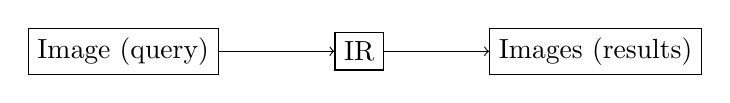
\begin{tikzpicture}
    \node[draw] (input) {Image (query)};
    \node[draw, rectangle, right of=input, node distance=3cm] (ir) {IR};
    \node[draw, right of=ir, node distance=3cm] (output) {Images (results)};
    \draw[->] (input) -- (ir);
    \draw[->] (ir) -- (output);
\end{tikzpicture}
\newline
We want a feature description system that is:
\begin{itemize}
    \item Translation invariant
    \item Rotation invariant
    \item Intensity invariant
    \item Scale invariant
\end{itemize}

A small portion of an image is called a \textbf{patch}.
We want to implement a pipeline that works like this:

% image -> feature detection -> feature description -> feature matching

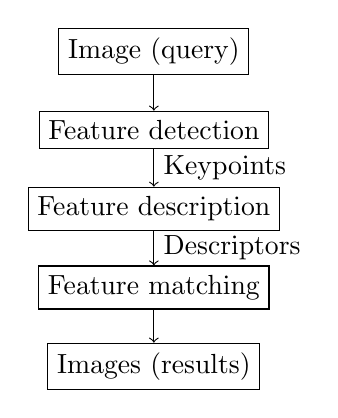
\begin{tikzpicture}
    \node[draw] (input) {Image (query)};
    \node[draw, rectangle, below of=input, node distance=1cm] (fd) {Feature detection};
    \node[draw, rectangle, below of=fd, node distance=1cm] (fdesc) {Feature description};
    \node[draw, rectangle, below of=fdesc, node distance=1cm] (fmatch) {Feature matching};
    \node[draw, below of=fmatch, node distance=1cm] (output) {Images (results)};
    \draw[->] (input) -- (fd);
    \draw[->] (fd) -- node[right] {Keypoints} (fdesc);
    \draw[->] (fdesc) -- node[right] {Descriptors} (fmatch);
    \draw[->] (fmatch) -- (output);
\end{tikzpicture}

\subsubsection{Feature detection}
\label{sec:feature_detection}

We want to detect points of interest (\textbf{keypoints}) in an image.
If we were to detect edges, we would have a problem because them are not descriptive enough.
If we were to detect corners, we would have a problem because they are not scale invariant.
We have to detect \textbf{blobs}.
A \textbf{blob} is a circular flat region of an image.

We can detect a simple blob using the \textbf{LoG} operator.
Depending on the $\sigma$ we choose, we can detect blobs of different sizes.
We normalize the LoG operator to remove the difference in scale depending on the $\sigma$ we choose.
Thus obtaining the \textbf{NLoG} operator $\sigma^2 LoG(x,y,\sigma)$.

Depending on the sigma we choose we detect different size blobs

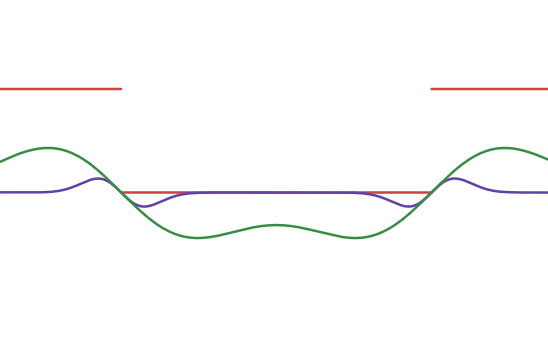
\includegraphics[width=0.3\textwidth]{assets/blob_0.png}
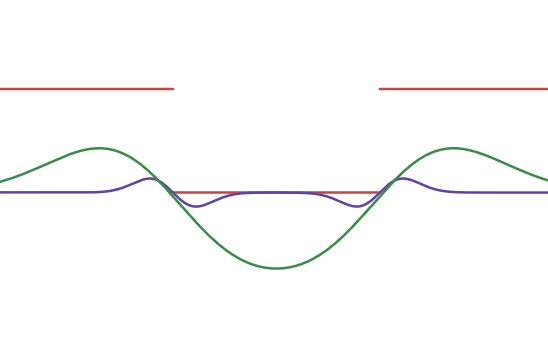
\includegraphics[width=0.3\textwidth]{assets/blob_1.png}
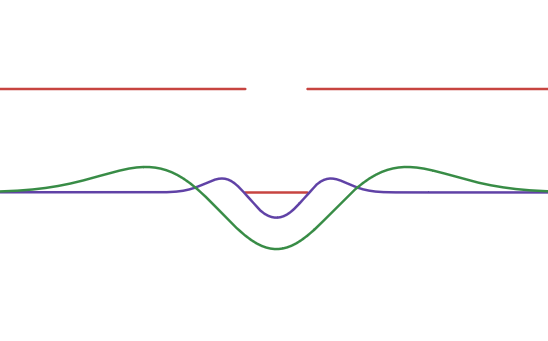
\includegraphics[width=0.3\textwidth]{assets/blob_2.png}

To obtain a description of blobs of each size we must check with different sigmas.
We use many different sigmas close to each other and we obtain a \textbf{scale space}.
The scale space can be expressed like this:
\[
    G[x,y,\sigma] \overset{\Delta}{=} (g[x,y,\sigma_1]*f[x,y], \dots, g[x,y,\sigma_n]*f[x,y])
\]
Usually $\sigma_i=s^i\sigma_1\text{ for }i=2,\dots,n$. Usually $\sigma_1=1.6$.
Usually $s$ is chosens such that $\sigma$ doubles every 2 steps. The number of steps
needed to double $\sigma$ is called octave.

Given a gaussian scale space representation $G[x,y,\sigma]$ the coordinates\\ $x^*,y^*,\sigma^*$ 
of its local minima correspond to keypoints $x^*,y^*$, $\sigma^*$ is called caracteristic scale.
How do we compute keypoints? Using the \textbf{NLoG} operator.
\[
    g_\sigma[x,y,\sigma] = \sigma\nabla^2g[x,y,\sigma] = \sigma LoG[x,y,\sigma]
\]

We want to find $\text{min}G[x,y,\sigma]$.
We will never use the LoG, because the cost is 4 1D convolutions.
If we compute the derivative of a gaussian filter w.r.t. $\sigma$ with the Taylor approximation
up to a factor, we get the following:
\[
    g_\sigma[x,y,\rho\sigma]-g[x,y,\sigma] \approx (\rho-1)NLoG[x,y,\sigma]
\]
This is a new operator called \textbf{Difference of Gaussians} (DoG).
We see that the difference between $g[x,y,\sigma_i]*f[x,y]$ and $g[x,y,\sigma_{i+1}]*f[x,y]$
is approximately $(s-1)$ times the NLoG operator.

We can easily define the DoG representation. 
If we have $G[x,y,\sigma]$ we define 
$D[x,y,\sigma] \overset{\Delta}{=} G[x,y,\sigma_{i+1}]-G[x,y,\sigma_i]\text{ for }0<i<n$
We want to find the local minima of the DoG representation, this is done by


\subsection{Feature description}
\label{sec:feature_description}

Once we have detected a keypoint $(x^*,y^*,\sigma^*)$ we need to describe it.
Let's call $f[x,y]*g[x,y,\sigma^*]=f[x,y\sigma^*]$ and a patch $P$ centered in $(x^*,y^*)$ with size $d$
$P[x,y,d]=\{[x,y]:dist_\infty((x,y),(x^*,y^*))\le d\}$

We can write a gradient as magnitude and orientation:
\[
    \nabla f[x,y,\sigma^*]=\begin{cases}
        ||\nabla f[x,y,\sigma^*]|| \\
        \alpha(\nabla f[x,y,\sigma^*])
    \end{cases}
\]

We take the patch centered in a keypoint with $d=2\lambda_1\sigma^*$ (typically $\lambda_1=4.5$)
and we have to find the "most important" gradient orientation.
We call this angle $\theta^*$.
To find this angle, for every pixel in the patch we compute the gradient and then
we build the orientation histogram.
We use $K_1=36$ bins and we divide the $[0,2\pi]$ range in $K_1$ bins.
We assign the bin $R=\left\lfloor \frac{K_1}{2\pi} \alpha(\nabla f[x,y,\sigma^*]) \right\rfloor$
to every pixel in the patch and we increment the corresponding bin in the histogram proportionally
to the magnitude of the gradient in that point.

\begin{figure}[H]
    \centering
    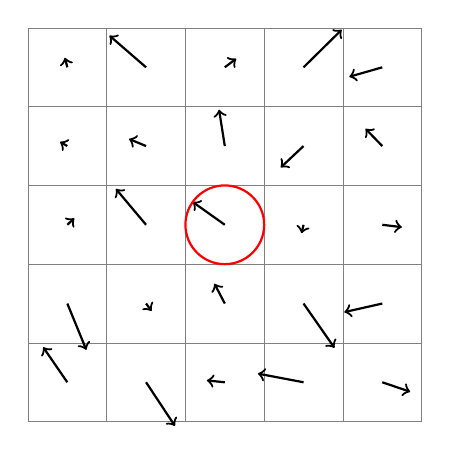
\begin{tikzpicture}
        \foreach \x in {0,1,...,4} {
            \foreach \y in {0,1,...,4} {
                \pgfmathsetmacro\angle{rand*360}
                \pgfmathsetmacro\length{0.4 + rand*0.3}
                \draw[gray, very thin] (\x, \y) rectangle (\x+1, \y+1);
                \draw[->, thick] (\x+0.5, \y+0.5) -- ++(\angle:\length);
            }
        }
        \draw[red, thick] (2.5, 2.5) circle (0.5);
    \end{tikzpicture}
    \caption{Patch with gradient arrows for each pixel. The red circle indicates the keypoint.}
    \label{fig:patch_gradients}
\end{figure}

\begin{figure}[H]
    \centering
    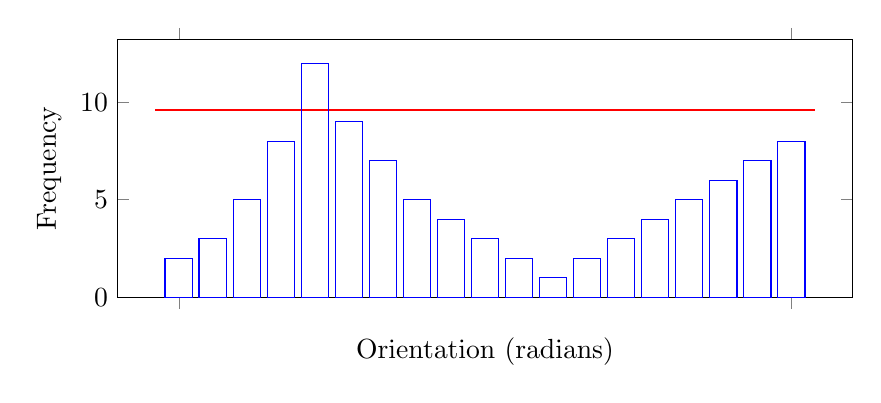
\begin{tikzpicture}
        \begin{axis}[
            ybar,
            xtick=data,
            x tick label style={rotate=90, anchor=east},
            ymin=0,
            ylabel={Frequency},
            xlabel={Orientation (radians)},
            width=0.9\textwidth,
            height=0.4\textwidth,
            xticklabels={},
        ]
        \addplot[red, line legend, sharp plot, nodes near coords={},
            update limits=false,shorten >=-3mm,shorten <=-3mm] 
        coordinates {(0,9.6) (18,9.6)};
        \addplot[blue] coordinates { 
            (0, 2) (1, 3) (2, 5) (3, 8) 
            (4, 12) (5, 9) (6, 7) 
            (7, 5) (8, 4) (9, 3) 
            (10, 2) (11, 1) (12, 2) 
            (13, 3) (14, 4) (15, 5) 
            (16, 6) (17, 7) (18, 8)
        };
        \end{axis}
    \end{tikzpicture}
    \caption{Orientation histogram for the gradients in the patch. The red dashed line indicates the threshold at 0.8 times the maximum bin value.}
    \label{fig:orientation_histogram}
\end{figure}

\begin{figure}[H]
    \centering
    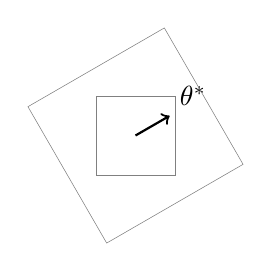
\begin{tikzpicture}
        % Draw the original patch
        \draw[gray, very thin] (0, 0) rectangle (1, 1);
        \draw[->, thick] (0.5, 0.5) -- ++(30:0.5) node[anchor=south west] {$\theta^*$};
        
        % Draw the rotated patch
        \begin{scope}[rotate around={30:(0.5,0.5)}]
            \draw[gray, very thin] (-0.5, -0.5) rectangle (1.5, 1.5);
        \end{scope}
    \end{tikzpicture}
    \caption{Original patch and rotated patch.}
    \label{fig:rotated_patch}
\end{figure}

If the new patch falls outside the image we \textbf{discard} the keypoint.

We select all the bins that are greater than 0.8 times the maximum value in the histogram.
We treat each of these bins as an individual keypoint and patch.

For each of these bins we rotate the patch such that the angle $\theta^*$ points to
the right. Actually this is done by counter-rotating the image by $\theta^*$.
Once we have counter-rotated the image we select a new patch of size $d=2\lambda_2\sigma^*$
(typically $\lambda_2=6$) on the new rotated image.

We call this new patch $P_{desc}$ and divide it into $N=4$ subpatches. For each subpatch we
compute a new orientation histogram using the gradient $\nabla f[\hat{x},\hat{y},\lambda_2\sigma^*]$ (where
the hat indicates the coordinates in the rotated image).
We use $K_2=8$ bins for this histogram. We obtain $N^2K_2$ values.

We call the vector of all these values the \textbf{feature vector} $\psi$.
This feature vector will be sparse, with most of the values being zero.

We clamp the values of the feature vector such that they are in the range $[0,0.2||\psi||]$
and we normalize the vector such that $||\psi||=512$.
Each component is quantized in 8 bits.
In this way the vector will be 128B.
The resulting vector is called \textbf{SIFT feature descriptor} corresponding to the keypoint
$(x^*,y^*)$
\subsection{Feature matching}
\label{sec:feature_matching}

Onc we have detected and described keypoints, we have a bunch of dense vectors in a high-dimensional space.
We call those vectors \textbf{embeddings}.

Once we have embeddings for all of our dataset, and an embedding for a query image, we want to find the closest
embeddings to the query image. Closeness can be either a distance or an angle.
This problem is called \textbf{nearest neighbor search}.

The easiest way to do this is the \textbf{brute force search}, where we test one by one all the embeddings in the dataset.
This algorithm has many problems:
\begin{itemize}
    \item It only outputs one result, not taking into account the rest of the dataset and any possible noise.
    \item It always outputs a result, even if the query image is not related to the dataset.
    \item It is slooooowwwwww.
\end{itemize}

We define a metric $NNDR(\phi_a, \phi_b^1, \phi_b^2)=\frac{d(\phi_a, \phi_b^1)}{d(\phi_a, \phi_b^2)}$ to use as threshold,
we do not output anything if NNDR is bigger than 0.8.

A greedy optimization is to use a bounding box to discard embeddings that are too far away from the query image (\textbf{KD-tree}).
The problem is that with the number of dimensions the number of intersections grows exponentially.

A better approach is to use \textbf{locality sensitive hashing (LSH)}.
In this approach we use hashing functions that have locality preserving properties
so that close points are hashed to close hash values.
LSH gives an approximate solution to the NNS problem.

\subsubsection{Vector quantization}

Also this approach is really slow and does not scale well with many items.

We use a technique called \textbf{vector quantization}.
Given our embeddings $\Psi=\{\psi_1, \dots, \psi_n\}$ and a set of vectors in the same 
space $C=\{\mu_1, \dots, \mu_k\}$ called \textbf{codebook},
we define a \textbf{vector quantizer} as a function $q_C:\Phi\rightarrow C | q_C(\phi)=argmin_{\mu\in C}||\psi-\mu||$

We define a tasselation of the space called \textbf{Voronoi tasselation} such that
each cell is $V_i={x\in\mathbb{R}|q_C(x)=\mu_i}$.

We want to use the optimal codebook that minimizes the reconstruction error $RE(C)=\sum_{i=1}^{n}||\phi_i-q_C(\phi_i)||$.
The problem is then formulated as $C^*=argmin_CRE(c)$.

We can use K-means to solve this problem.

To actually use the system we then translate each vector in $C^*$ in its index,
we call this index the \textbf{visual term-id}.
Then we can use the usual inverted index.
\subsection{Convolutional Neural Networks}
\label{sec:convolutional_neural_networks}

To be effective in tasks like object recognition, image classification, semantic segmentation and object localization
we need to use a \textbf{Convolutional Neural Network (CNN)}.

\subsubsection{Difference between convolution and cross-correlation}

In a neural network a convolutional layer is a generalization of the convolution:
\[
    f*g:\mathbb{Z}^d->\mathbb{R}^{d\ge1}
\]\[
    f[u]*g[u]=\sum_{v\in\mathbb{Z}^d}f[v]g[u-v]
\]

The cross-correlation is defined as:
\[
    f \circledast g:\mathbb{Z}^d->\mathbb{R}^{d\ge1}
\]\[
    f[u] \circledast g[u]=\sum_{v\in\mathbb{Z}^d}f[v]g[v+u]
\]

We see that the only difference is the sign of the shift.
We can prove that
\[
    f[u] \circledast g[u] = f[-u] * g[u]
\]
by changing the variable $u$ to $-w$.
With symmetric filters the two operations are equivalent.

\subsubsection{From MLP to CNN}

Why do we need CNNs? If we use a fully connected layer
it must have a number of parameters equal to
$(I+1) \times O$ where $I$ is the input size
and $O$ is the output size (weight matrix + bias).
With an average image of 1024x1024 pixels we would have
$I=1048576$ and with any non trivial $O$ we get a huge amount
of parameters.

We have to apply the principles used in image processing to 
make the network more efficient.
Let's call the weights of the layer $W$, the input $f$, the output $z$ and the bias $b$.
In a linear layer we have:
\[
    z[x,y]=\sum_{k}\sum_{l}W[x,y,k,l]f[k,l]+b[x,y]
\]
We can rewrite this as:
\[
    z[x,y]=\sum_{u}\sum_{v}\hat{W}[x,y,u,v]f[x+u,y+v]+b[x,y]
\]

\begin{itemize}
    \item \textbf{Translation invariance}: $\hat{W}[x,y,u,v]=\hat{W}[u,v]$
    \item \textbf{Spatial locality}: A pixel at $(x,y)$ has to depend only on
    pixels near it. We only take into account a patch $P = D\times D$ around the pixel.
    $z[x,y]=\sum_{u,v\in P}\hat{W}[u,v]f[x+u,y+v]+b[x,y]$
\end{itemize}
The resulting formula needs only $D^2+1$ parameters and
is actually a convolutional layer.

When we have multiple channels we need a 3D tensor instead of a 2D matrix.
On GPU the performance is not affected significantly by the number of channels.
The new formula is:
\[
    z[c_0,x,y]=\sum_c\hat{W}[c_0,c,x,y]\circledast f[c,x,y]+b[c_0,c]
\]

\subsection{CNN architectures}
\label{sec:cnn_architectures}

With more layers the computational cost increases, we need to find some techniques to reduce it.
One of those is \textbf{striding}: instead of computing the convolution at every pixel, we skip some pixels.
A priori in convolutional networks there is no concept of scale, to introduce it we use \textbf{pooling}.
Pooling is a non trainable transformation that reduces the size of the input.

The pooling operation divides the input into patches and applies a function to each patch.
The most common pooling function is the max pooling, that takes the maximum value for each patch.
Another pooling function is the average pooling, that takes the average value for each patch.

Patches can overlap or not, and be as complex as we want.
Pooling is always a down-sampling operation.

With smaller images convolutions take less time to compute.

In computer vision we have 3 types of tasks:

\begin{itemize}
    \item \textbf{Image classification}: We have an image and we want to know what's in it.
    \item \textbf{Object detection}: We have an image and we want to know where the objects are. 
    For example \textbf{You Only Look Once (YOLO)} is a network that does object detection.
    It divides the image into a grid of cells (patches) and for each cell detects if there is an object and of what class.
    \item \textbf{Semantic segmentation}: We have an image and we want to know what's in it and where.
    We want to do pixel-wise object detection. First we downsample the image to classify it then we use 
    upsampling to get back to the original image size with each pixel classified.
\end{itemize}

\subsubsection{LeNet}
\label{sec:lenet}

This network was used for digit recognition (MNIST dataset).

\begin{itemize}
    \item Input: $32\times32$ pixels ($1024$ pixels)
    \item Convolutional layer: $5\times5$ kernel, $6$ filters, $1$ stride
    \item ReLU activation with input size $28\times28\times6$
    \item Pooling layer: $2\times2$ kernel, $2$ stride
    \item Convolutional layer: $5\times5$ kernel, $16$ filters, $1$ stride
    \item ReLU activation with input size $10\times10\times16$
    \item Pooling layer: $2\times2$ kernel, $2$ stride
    \item Flatten layer that outpus a dense embedding of size $400$
    \item MLP that does the required task
\end{itemize}

Why bother with all these convolutional layer and not stop with 2 linear layers?
It's true that with two linear layers we can approximate any function, but the number of parameters
grows exponentially with the complexity of the function.

A manifold in two dimensions is a curve, in three dimensions is a surface, in four dimensions is a volume etc.
It's a subspace of the input space where the valid images lie.
We say that a valid image can be represented on a low dimensional manifold because only a small subset of all possible images
are valid.




\section{Language models}
\subsection{Language Models}
\label{sec:language_models}

\subsubsection{Statistical Machine Learning}

In statistical machine learning we need:
\begin{itemize}
    \item a \textbf{training corpus} $\mathcal{T}={(d_1,y_1),\dots,(d_m,y_m)}$.
    \item a \textbf{representation funciton} $\phi:D\rightarrow\mathbb{R}^n$, this
    function has to map each $d_i$ to it's corresponding $y_i$.
    \item to choose our \textbf{hypothesis class} $\mathcal{H}\in{f_1, f_2, \dots}$. It can be written like
    $f(\phi(d_i)|\Theta)=\hat{y_i}(\Theta)$. Where $\Theta$ are the parameters
    of the model. We usually chose an arbitrary hypothesis class and then we
    check if its output is good enough.
    \item an \textbf{error function} $\mathcal{L}(\Theta)=\sum_i e(y_i,\hat{y_i})$.
    \item to find a value of $\Theta$ to minimize $\mathcal{L}$.
\end{itemize}

\subsubsection{Definitions}

\begin{itemize}
    \item \textbf{Vocabulary}: a finite set of something, denoted as $V$.
    The elements that we will denote as $w\in V$ are called \textbf{words}.
    \item \textbf{Sentence}: a sequence of $n$ words in $V$ denoted as $s=w_1,\dots,w_n$.
    We denote with $V^+$ the infinite set (but numerable) of all finite sentences over 
    $V$ (not necessarily grammatically correct).
    \item \textbf{Language model}: a language model over $V^+$ is a function $P:V^+\rightarrow\mathbb{R}$
    s.t. $\forall s\in V^+$ we have $P[s]\geq 0$ and $\sum_{s\in V^+}P[s]=1$. This is a probability distribution
    over $V^+$.
\end{itemize}

From now on $P[s]$ is a number $\in[0,1]$ while $P(s)$ is a probability distribution where $s$ denotes a random variable
over $V^+$. We will also uso $P[w]$ and $P(w)$ to denote the same thing as before but with single word sentences.

$V^+$ is infinite so we cannot store it, we have to approximate it with $\mathcal{T}$.
\begin{figure}[H]
    \centering
    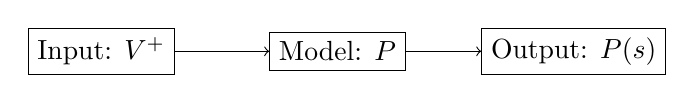
\begin{tikzpicture}
        \node (input) [draw, rectangle] {Input: $V^+$};
        \node (model) [draw, rectangle, right of=input, node distance=3cm] {Model: $P$};
        \node (output) [draw, rectangle, right of=model, node distance=3cm] {Output: $P(s)$};
        
        \draw[->] (input) -- (model);
        \draw[->] (model) -- (output);
    \end{tikzpicture}
    \caption{The ideal model.}
    \label{fig:language_model}
\end{figure}

\begin{figure}[H]
    \centering
    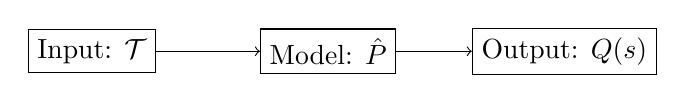
\begin{tikzpicture}
        \node (input) [draw, rectangle] {Input: $\mathcal{T}$};
        \node (model) [draw, rectangle, right of=input, node distance=3cm] {Model: $\hat{P}$};
        \node (output) [draw, rectangle, right of=model, node distance=3cm] {Output: $Q(s)$};
        
        \draw[->] (input) -- (model);
        \draw[->] (model) -- (output);
    \end{tikzpicture}
    \caption{The approximate model.}
    \label{fig:approximated_language_model}
\end{figure}

A vocabulary can contain all possible words in a language
but it can also have some missing, in that case we add a special word $<OOV>$ to represent
all the words that are not in the vocabulary.

How close is $Q(s)$ to $P(s)$?

If we use the model for a \textbf{downstream task} we need to evaluate the model on the specific task that
it will be used for.

To evaluate a model in general we need an evaluation corpus $\mathcal{E}$ that is
still a subset of $V^+$ and has a very small intersection with $\mathcal{T}$.

Let's say that an evaluation corpus is composed of $n$ sentences $s_1,\dots,s_n$.
We concatenate all the sentences to form a single huge sentence $w_1,\dots,w_T$.
The \textbf{perplexity} of the model $P$ over $w_1,\dots,w_T$ is defined as:
\[
    PP(w_1,\dots,w_T)=P[w_1,\dots,w_T]^{-\frac{1}{T}}
\]
\[
    P[w_1,\dots,w_T]=P[w_1]\prod_{i=2}^{T}P[w_i|w_1,\dots,w_{i-1}]
\]
\[
    PP(w_1,\dots,w_T)=\left(P[w_1]\prod_{i=2}^{T}P[w_i|w_1,\dots,w_{i-1}]\right)^{-\frac{1}{T}}
\]

This is the \textbf{geometric mean} of the inverse of the probability of each word in the sentence.

What is $P[w_i|w_1,\dots,w_{i-1}]$? It's the probability of seeing
the word $w_i$ given the previous part of the sentence.

The perplexity measures how overall the number of choices has been reduced
while generating the sentence. How many words on average are
probable (with non 0 probability) given a starting sentence.

In English the perplexity is tought to be arount 15 and 20.

If we consider the \textbf{uniform language model} where $P[w_i|w_1,\dots,w_{i-1}]=\frac{1}{|V|}$ 
(the words are all equally probable and independent) we have:
\[
    P[w_1,\dots,w_T]=\left(\frac{1}{|V|}\right)^T
\]
\[
    PP(w_1,\dots,w_T)=|V|
\]
This makes sense as we randomly choose a word from $V$ at each step.

We have to mark the start and the end of the sentence with special words $<s>$ and $</s>$.
To take this into account we would have to modify the perplexity formula (would be a bit nicer).
These two words are ignored for the rest of the notes.

At this point we can use a model to generate a sentence.

Given a starting sentence $w_1,\dots,w_n$ we want to generate $\hat{w_1},\dots,\hat{w_m}$.
We can find $\hat{w_1}$ as $\hat{w_1}=\text{argmax}_{w\in V}P[w|w_1,\dots,w_n]$.
Then we can append $\hat{w_1}$ to the sentence and repeat the process until we reach the end of the sentence.
This is called \textbf{greedy search}.

\subsection{N-Gram language models}
\label{sec:n_gram_language_models}

\subsubsection{Evaluating language models}

We want to know how close $P(s)$ is to $Q(s)$.
We want to calculate the $\mathcal{L}(P,Q)$. The language learning problem is to find $\text{argmin}_Q\mathcal{L}(P,Q)$.
We need to define $\mathcal{L}$ that takes as input two probability distributions on the same set of events and returns a number.
In the '48 Shannon was studying what information a probability distribution carries.
If we have a measure of information, if it does not change the measure is useless. We are interested in changes, in strange
events. We can measure the "interestingness" of something looking at its probability distribution.
Something that is always happening is boring, something that rarely happens is the most interesting.

\begin{figure}[H]
    \centering
    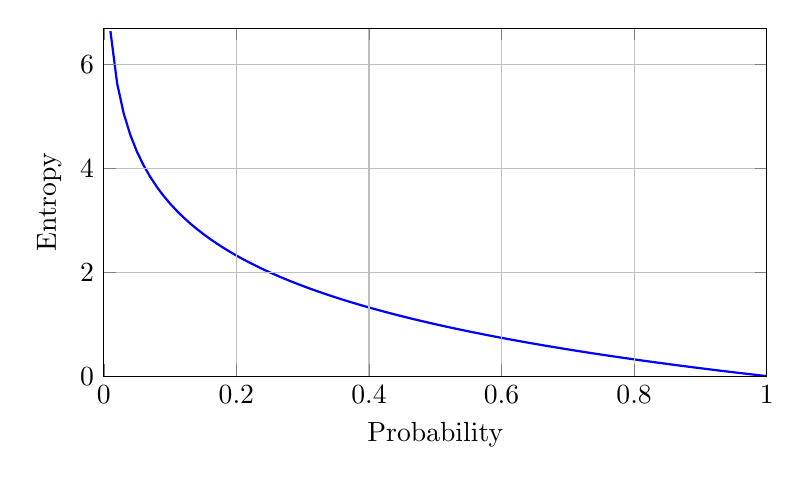
\begin{tikzpicture}
        \begin{axis}[
            xlabel={Probability},
            ylabel={Entropy},
            xmin=0, xmax=1,
            ymin=0, ymax=6.7,
            domain=0.01:1,
            samples=100,
            ytick={0,2,4,6},
            xtick={0,0.2,0.4,0.6,0.8,1},
            grid=major,
            width=10cm,
            height=6cm,
            enlargelimits=false,
            clip=false,
            axis on top,
        ]
        \addplot[blue, thick] {-ln(x)/ln(2)};
        \end{axis}
    \end{tikzpicture}
    \caption{Entropy vs Probability}
    \label{fig:entropy_vs_probability}
\end{figure}

The information content or entropy is defined as
\[
    I[x]=-log(P[x])
\]

We usually calculate the expected value of the information on a 
random variable like this:
\[
    H(X)=E[I(X)]=E[-log(X)]=\sum_{x\in\mathcal{X}}P[x]log(P[x])
\]

If we use the base $e$ we call the unit of measure of $I$ \textbf{nat},
if we use the base 2 we call it \textbf{bit}.

$H$ has some interesting properties:
\begin{itemize}
    \item $H(P) \geq 0$.
    \item $H(P) \leq log(|\mathcal{X}|)$
    \item $H(P)=0 \iff \exists x\in\mathcal{X}:P[x]=1$
    \item $P(P)=log(|\mathcal{X}|) \iff \forall x\in\mathcal{X}:P[x]=\frac{1}{|\mathcal{X}|}$
\end{itemize}

We want to know how much information do we loose if we use
$Q$ instead of $P$.
To do this we use
\[
    H(P,Q)=-\sum_{x\in\mathcal{X}}P[x]log(Q[x])
\]
This is called the \textbf{cross-entropy}.
We leave $P$ because it govern how things actually happen,
we replace $Q$ because that's what governs the information
we have about the world.

(The professor makes an example of what is the interestingness of him
throwing a shoe to a student, even if we don't know the probability
we can approximate an information content that's very high).

With cross entropy we can calculate how much information
we lose (we always lose information with an approximation)
w.r.t. the real world.

The \textbf{Kullback-Leibler divergence} is defined as
\[
    D_{KL}(P||Q)=H(P,Q)-H(P)=-\sum_{x\in\mathcal{X}}P[x]log\left(\frac{Q[x]}{P[x]}\right)
\]

Keep in mind that the divergence is not symmetric:
\[
    D_{KL}(P||Q)\neq D_{KL}(Q||P)
\]
A very important property of the $D_{KL}$ is the
inequality of Gibbs:
\[
    D_{KL}(P||Q)\geq 0
\]

If $P=Q$ then $D_{KL}(P||Q)=0$.

To get back the entropy of sentences we need to normalize
the entropy by the length of the sentence.
$V^+_n$ is the set of all sentences of length $n$,
its cardinality is $|V^+_n|=|V|^n$.
It makes sense to compute the $I[s_n]$ and $H[s_n]$.
The \textbf{entropy rate} is $\bar{H}(s_n)=1/nH[s_n]$.

The entropy of a \textbf{language model} is the limit
of the entropy rate
\[
    H(P)=\lim_{n\rightarrow\infty}\bar{H}(s_n)
\]
And the \textbf{cross-entropy} is
\[
    H(P,Q)=\lim_{n\rightarrow\infty}\frac{1}{n}\sum_{x\in V^+_n}P[s_n]log(Q[s_n])
\]
It makes sense to compute the $D_{KL}$.

The most important theorem in LM theory is the
\textbf{Shannon-McMillan-Breiman theorem}:
Suppose that $P(s)$ and $Q(s)$ are \textbf{good} language models,
knowing the definitions of $V^+,V^+_n,H(P),H(P,Q)$.
$\sigma_n\in V^+_n$ is a single specific element of $V^+_n$.
Then
\[
    H(P,Q)=-\lim_{n\rightarrow\infty}\frac{1}{n}log(Q[\sigma_n])\approxeq
    -\frac{1}{n}log(Q[\sigma_n]) \text{for large enough } n
\]

The first problem that appears is the definition of "\textbf{good}".
In the original theorem stated \textbf{ergodic} and \textbf{stationary}.
\textbf{Stationary} means that the property of the subsequences don't change
independently of their position.
\textbf{Ergodic} basically means that the time average is 
equal to the expectation.
Essentially $n$ should be large enough to see every word in $V$
and appreciate their probability.

Our real value of $n$ is not infinite so we have an approximation.
The sequence $\sigma_n$ that we will use to compute $Q$ is the training corpus $\mathcal{T}$

So given a corpus $\mathcal{T}$ we can compute $H(P,Q)$:
\[
    H(P,Q)=-\frac{1}{T}log(Q[w_1,\dots,w_T])
\]

Remember that the perplexity is defined as
\[
    PP(w_1,\dots,w_T)=exp(log(Q[w_1,\dots,w_T]^{-\frac{1}{T}}))
\]
\[
    =exp(-\frac{1/T}Q[w_1,\dots,w_T])
\]
\[
    =e^{H(P,Q)}
\]

So now we need to solve
\[
    \text{argmin}_Q\mathcal{L}(P,Q)
\]
\[
    =\text{argmin}_Q D_{KL}(P||Q)
\]
\[
    =\text{argmin}_Q H(P,Q)-H(P)
\]
Because $H(P)$ is constant
\[
    =\text{argmin}_Q H(P,Q)
\]
And with the Shannon-McMillan-Breiman theorem we can approximate
to
\[
    \approxeq \text{argmin}_Q -\frac{1}{T}log(Q[w_1,\dots,w_T])
\]

In some scenarios we want to learn 
\[
    P(w|w_1,\dots,w_{n-1})=\begin{cases}
        1 & \text{if } w=w_i\\
        0 & \text{otherwise}
    \end{cases}
\]
This is the word prediction problem.
So it's
\[
    \text{argmax}_Q log(Q[w_T|w_1,\dots,w_{T-1}])
\]

Now we have an estimate of the probability and we can use it
to generate new sentences.

\subsubsection{N-gram models}

An n-gram is a sequence of $n$ words.
The $n$ order Markov assumption is:
Suppose $s\in V^+$, then each word $w\in s$ only depends on the previous $n-1$ words.
\[
    P[s]=P[w_1,\dots,w_n]=\prod_{i=1}^{T}P[w_i|w_{i-1},\dots,w_{i-n+1}]
\]
This is somewhat unrealistic but makes the problem tractable.
Using this assumption we can propose some models:
\begin{itemize}
    \item \textbf{Unigram model}: $P[w_1,\dots,w_k]=\prod_{i=1}^{k}P[w_i]$
    In this case it's very easy to estimate the probabilities with the
    frequencies in the training corpus. This model dos not take into account
    co-occurrences of words.
    \item \textbf{Bigram model}: $P[w_1,\dots,w_k]=\prod_{i=1}^{k}P[w_i|w_{i-1}]$
    \item \textbf{Trigram model}: $P[w_1,\dots,w_k]=\prod_{i=1}^{k}P[w_i|w_{i-1},w_{i-2}]$
    \item and so on...
\end{itemize}

With $n$ growing the training corpus might not contain a certain n-gram.
To solve this we can use \textbf{smoothing} techniques.

Laplace smoothing is the simplest one: "add one to each count".
\[
    P[w_i|\dots]=\frac{C[w_i,\dots]+1}{C[\dots]+|V|}
\]

If we want to use a machine learning model to estimate the 2-gram probabilities we need to
calculate a square matrix $W$ of size $|V|\times|V|$ with all the counts.
To each word $w\in V$ we associate a one-hot vector $x\in Z^{1\times |V|}$.
In $x$ all the elements are 0 except the one corresponding to $w$ (in lexicographic ordering) that is 1.
What is $xW$? It's the row of $W$ corresponding to $w$.

\[
    P[w_i w_j]=\frac{W_ij}{\sum_{j=1}^{|V|}W_ij}
\]

We want to learn this matrix instead of computing it by hand.
We can use a linear layer with weight matrix $\hat{W}$ and learn it, this is an estimate of $W$.
The model is $y=x\hat{W}$. What is $y$? With $\hat{W}$ randomly initialized we get some positive and negative numbers as output.
To get only positive numbers we can use $y=exp(x\hat{W})$. So
$z=(e^{\hat{W}_i1},\dots,e^{\hat{W}_i|V|})$. These are in some way our estimate of the counts.
We call $x\hat{W}$ the \textbf{logits} (logarithm of the counts).
To calculate the probability from the counts we get $P[w_i|w_i]=\frac{z_j}{\sum_{i=1}^{|V|}z_i}$.
This function is called \textbf{softmax}.

Our neural network will be:

\begin{figure}[H]
    \centering
    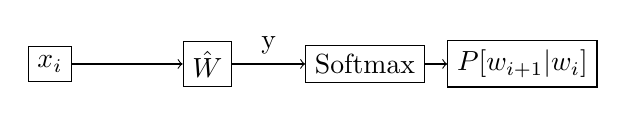
\begin{tikzpicture}[node distance=2cm, auto]
        % Nodes
        \node (input) [draw, rectangle] {$x_i$};
        \node (weights) [draw, rectangle, right of=input] {$\hat{W}$};
        \node (softmax) [draw, rectangle, right of=weights] {Softmax};
        \node (output) [draw, rectangle, right of=softmax] {$P[w_{i+1}|w_i]$};

        % Edges
        \draw[->] (input) -- (weights);
        \draw[->] (weights) -- node[midway, above] {y} (softmax);
        \draw[->] (softmax) -- (output);
    \end{tikzpicture}
    \caption{Neural network for estimating $P[w_{i+1}|w_i]$}
    \label{fig:neural_network}
\end{figure}

We can calculate the loss function
\[
    \mathcal{L}=-\frac{1}{\mathcal{T}}\sum_{i=1}^{|\mathcal{T}|}log(P[w_{i+1}|w_i])
\]

The number of parameters of this model is $|V|^2$. 
If we used a trigram model we would have $|V|^3$ parameters.
This is a lot of parameters, especially considering that $|V|$ is 
in the order of $10^6$. 

A bigram model is quite shitty, and also consumes a lot of memory.
\subsection{Feed forward language models}
\label{sec:feed_forward_language_models}

The problem with the n-gram model is that the size of the weight matrix grows exponentially with $n$.
Most of the probabilities in this model are useless and are zero (LeCun).

Yoshua Bengio et al. in 2003 proposed a neural network called \textbf{feedforward neural network language model}.

This network uses embeddings to represent words. A word embedding is $e: V\rightarrow\mathbb{R}^{1\times d}$.
To process word embeddings we need a matrix $E$ of size $|V|\times d$, this is called the \textbf{embedding matrix}.

We do not know what is the best embedding matrix $E$ so we need to learn it (we start with a random matrix).

To get a word embedding out of $E$ we just compute $e=wE$ where $w$ is the one-hot vector of the word.
This step can be optimized by getting only the row of $E$ corresponding to the word but the result is the same.
$E$ will be composed by 
\[
    E=\begin{bmatrix}
        e_1 \\
        \vdots \\
        e_{|V|}
    \end{bmatrix}
\]

(For all the lectures the bias is omitted for simplicity but without loss of generality).

The feedforward layer is:
\begin{itemize}
    \item Given an activation function $\sigma$
    \item Given a linear layer $y=xW$ with $W\in\mathbb{R}^{n\times m}$
\end{itemize}

A feedforward layer is a parametrized function $f(\cdot|\Theta)$
s.t. $f(x|\Theta)=y=\sigma(xW)$.

We can write the language model $P[w_i|w_{i-1},\dots,w_{i-n+1}]$ as \\
$f(w_{i-1},\dots,w_{i-n+1})\rightarrow\mathbb{R}^{|V|}$.

This function will be actually $|V|$ functions $g(e(w_{i-1}),\dots,e(w_{i-n+1}))\rightarrow\mathbb{R}$.
$g$ takes the embeddings of the words and returns a real number.
\[
    g: \mathbb{R}^{(n-1)\times d}\rightarrow\mathbb{R}
\]
To implement $g$ we use an embedding layer $E$ and a feedforward layer.
To get a vector from all the embeddings we just concatenate them so that we can feed them to the FF layer.

The input of the FF layer will be $x_{i-1}E | \dots | x_{i-n+1}E = x$ where $x_{i}$ the one-hot vector of the word $w_i$.
So the output of the FF layer will be $y=\sigma(xW)$ where $W\in\mathbb{R}^{(n-1)d\times h}$.
$h$ is a hidden embedding dimension, we choose it.

\begin{figure}[H]
    \centering
    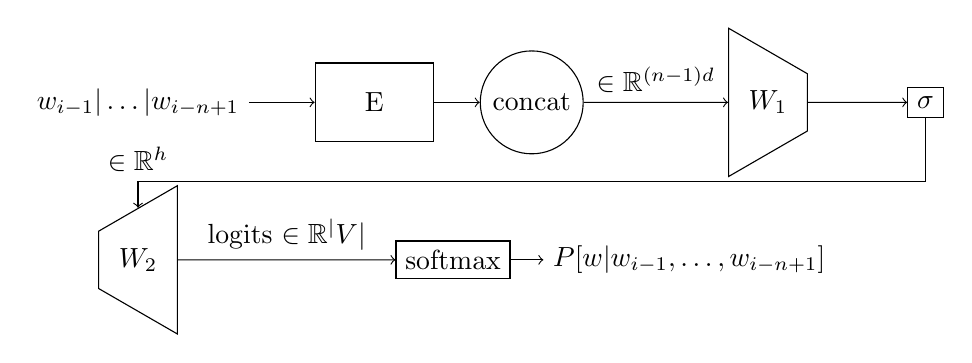
\begin{tikzpicture}[node distance=2cm, auto]
        % Nodes
        \node (input) { $w_{i-1}|\dots|w_{i-n+1}$ };
        \node (E) [draw, rectangle, minimum width=1.5cm, minimum height=1cm, right of=input, node distance=3cm] {E};
        \node (concat) [draw, circle, right of=E, node distance=2cm] {concat};
        \node (W1) [draw, trapezium, shape border rotate=270, trapezium left angle=60, trapezium right angle=60, minimum width=1.5cm, minimum height=1cm, right of=concat, node distance=3cm] {$W_1$};
        \node (sigma) [draw, rectangle, right of=W1, node distance=2cm] {$\sigma$};
        \node (W2) [draw, trapezium, shape border rotate=90, trapezium left angle=60, trapezium right angle=60, minimum width=1.5cm, minimum height=1cm, below of=input, node distance=2cm] {$W_2$};
        \node (softmax) [draw, rectangle, right of=W2, node distance=4cm] {softmax};
        \node (output) [right of=softmax, node distance=3cm] {$P[w|w_{i-1},\dots,w_{i-n+1}]$};
        
        % Edges
        \draw[->] (input) -- (E);
        \draw[->] (E) -- (concat);
        \draw[->] (concat) -- node[above] {$\in\mathbb{R}^{(n-1)d}$} (W1);
        \draw[->] (W1) -- (sigma);
        \draw[->] (sigma) |- +(0,-1) -| node[above] {$\in\mathbb{R}^h$} (W2);
        \draw[->] (W2) -- node[above] {logits $\in\mathbb{R}^|V|$} (softmax);
        \draw[->] (softmax) -- (output);
    \end{tikzpicture}
    \caption{Neural Language Model Architecture}
    \label{fig:neural_language_model}
\end{figure}

This model is a significant improvement over the n-gram model:
while we had $O(|V|^n)$ parameters in the n-gram model, we have $O(|V|nd+hd)$ parameters in the FF model.

The problem that we still have is that the $n$ parameter is fixed so
if we have a context bigger than $n$ we cannot use this model.
\subsection{Learning embeddings}
\label{sec:learning_embeddings}

If we have two words $w_i$ and $w_j$ represented with one-hot encoded vectors $x_i$ and $x_j$ we can
compute te cosine similarity between the two words as follows:
\[
    \cos(w_i,w_j)=\frac{x_i\cdot x_j}{\|x_i\|\|x_j\|}
\]
This approach returns always 0 for different words so it's not that useful.
With word embeddings we can compute the cosine similarity between two words as follows:
\[
    \cos(w_i,w_j)=\frac{x_iE\cdot x_jE}{\|x_iE\|\|x_jE\|}
\]

Why instead of learning a full neural network we don't just learn the embeddings?
In linguistics there is a concept called \textbf{distributional hypothesis} that states
that words that appear in the same context have similar meanings.
The idea is to learn similar embeddings for words that appear in the same context.

In 2023 Mikolov et al. proposed the \textbf{word2vec} model.

\subsubsection{Continuous bag of words (CBOW) model}

We start with a \textbf{center word} $w_c$ and a context of $2m$ words (symmetric window of size $m$).

The model is:
\[
    P[w_c|w_{c-m},\dots,w_{c-1},w_{c+1},\dots,w_{c+m}]=f(w_c)
\]
(the order of the context words does not matter).

For each one-hot encoded word $x_i$ we compute its embedding $e_i=x_iE$. ($E$ is the learnable embedding matrix).

For each center word $w_c$ we compute the centroid of the context words embeddings:
\[
    h=\frac{1}{2m}\sum_{-m\leq j\leq m,j\neq 0}e_{c+j}
\]
Then with a linear layer we compute the probability distribution over the vocabulary:
\[
    P[w_c|w_{c-m},\dots,w_{c-1},w_{c+1},\dots,w_{c+m}]=\text{softmax}(hW)
\]

\begin{figure}[H]
    \centering
    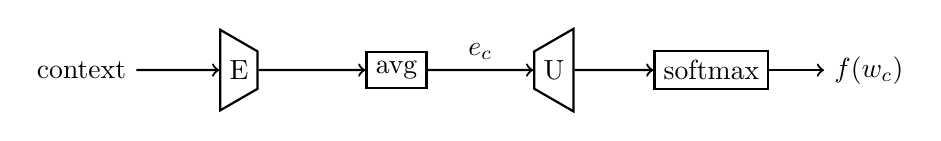
\begin{tikzpicture}[node distance=2cm, auto, thick]
        % Nodes
        \node (input) {context};
        \node (E) [trapezium, trapezium left angle=60, trapezium right angle=60, shape border rotate=270, draw, right of=input] {E};
        \node (avg) [draw, rectangle, right of=E] {avg};
        \node (linear) [trapezium, trapezium left angle=60, trapezium right angle=60, draw, shape border rotate=90, right of=avg] {U};
        \node (softmax) [draw, rectangle,right of=linear] {softmax};
        \node (output) [right of=softmax] {$f(w_c)$};

        % Edges
        \draw[->] (input) -- (E);
        \draw[->] (E) -- (avg);
        \draw[->] (avg) -- node[above] {$e_c$} (linear);
        \draw[->] (linear) -- (softmax);
        \draw[->] (softmax) -- (output);
    \end{tikzpicture}
    \caption{CBOW model architecture}
    \label{fig:cbow_model}
\end{figure}

The weights of the model are $O(2d|V|)$ and do not depend on the context size.
Calculating the softmax is unfortunately too expensive because it depends on $|V|$.

To solve this problem we use \textbf{contrastive learning}.

\subsubsection{Skip-gram model}

In the skip-gram model we do the opposite of the CBOW model.
Given a center word $w_c$ we want to predict the context words.
\[
    P(w_{c-m},\dots,w_{c-1},w_{c+1},\dots,w_{c+m}|w_c)
\]

To make this problem practical we need to use the na\"ive Bayes assumption:
\[
    P(w_{c-m},\dots,w_{c-1},w_{c+1},\dots,w_{c+m}|w_c)=\prod_{-m\leq j\leq m,j\neq 0}P(w_{c+j}|w_c)
\]

The na\"ive Bayes assumption gives us conditional independence, that is
different from complete independence.
Given the center word $w_c$ the context words are independent from each other.

Our model will learn to predict the probability distribution of the context words given the center word:
\[
    P(w_{c-m},\dots,w_{c-1},w_{c+1},\dots,w_{c+m}|w_c)
\]
\[
    =f(w_{c-m})\dots f(w_{c-1})f(w_{c+1})\dots f(w_{c+m})
\]

\begin{figure}[H]
    \centering
    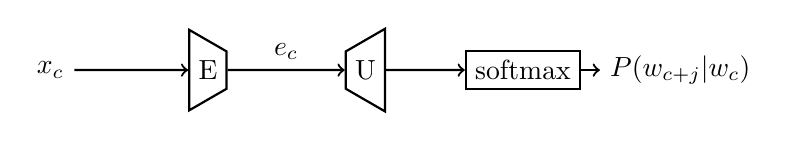
\begin{tikzpicture}[node distance=2cm, auto, thick]
        % Nodes
        \node (input) {$x_c$};
        \node (E) [trapezium, trapezium left angle=60, trapezium right angle=60, shape border rotate=270, draw, right of=input] {E};
        \node (linear) [trapezium, trapezium left angle=60, trapezium right angle=60, draw, shape border rotate=90, right of=E] {U};
        \node (softmax) [draw, rectangle,right of=linear] {softmax};
        \node (output) [right of=softmax] {$P(w_{c+j}|w_c)$};

        % Edges
        \draw[->] (input) -- (E);
        \draw[->] (E) -- node[above] {$e_c$} (linear);
        \draw[->] (linear) -- (softmax);
        \draw[->] (softmax) -- (output);
    \end{tikzpicture}
    \caption{Skip-gram model architecture}
    \label{fig:skip_gram_model}
\end{figure}

The loss will be:
\[
    \mathcal{L}=-\frac{1}{T}\sum_{c=1}^{T}\sum_{-m\leq j\leq m,j\neq 0}\log f(w_{c+j})
\]

The problem is the same as before: the softmax and the loss are too expensive.



\subsection{Recurrent neural networks}
\label{sec:recurrent_neural_networks}

The problem with the feedforward language model is that it has a fixed window size.
We can use a \textbf{recurrent neural network} to solve this problem.

The idea is to summarize every new word the model sees in a \textbf{hidden state}.
Then the model will use this hidden state to predict the next word.
\[
    P[w_{i+1}|w_1,\dots,w_i]=P[w_{i+1}|h_i]
\]
Where $h_i$ is the hidden state of the model up to position $i$.

The hidden state is computed as:
\[
    h_i=f(e_i,h_{i-1})
\]
($e_i$ is the embedding of the word $w_i$).

In this context we usually speak about time step $t$ instead of position $i$.

\begin{figure}[H]
    \centering
    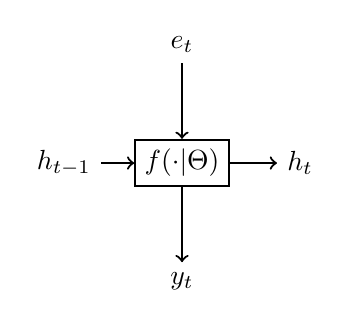
\begin{tikzpicture}[node distance=1.5cm, auto, thick]
        % Nodes
        \node (f) [draw, rectangle] {$f(\cdot|\Theta)$};
        \node (h_old) [left of=f] {$h_{t-1}$};
        \node (e) [above of=f] {$e_t$};
        \node (h) [right of=f] {$h_t$};
        \node (y) [below of=f] {$y_t$};

        % Edges
        \draw[->] (h_old) -- (f);
        \draw[->] (e) -- (f);
        \draw[->] (f) -- (h);
        \draw[->] (f) -- (y);
    \end{tikzpicture}
    \caption{RNN cell}
    \label{fig:rnn_cell}
\end{figure}

The RNN is a parametrized learnable function $f(\cdot|\Theta)$ s.t.
\[
    f(e_t,h_{t-1}|\Theta): \mathbb{R}^{1\times d}\times\mathbb{R}^{1\times h}\rightarrow\mathbb{R}^{1\times h}\times\mathbb{R}^{1\times m}
\]

$f$ is called the \textbf{RNN cell}.

Given a RNN cell, a sequence of $n$ words $w_1,\dots,w_n$ and their embeddings $e_1,\dots,e_n$ and $h_0=0$
we can compute the hidden states and the output of the model as follows:
\[
    h_t,y_t=f(e_t,h_{t-1}|\Theta)
\]

\begin{figure}[H]
    \centering
    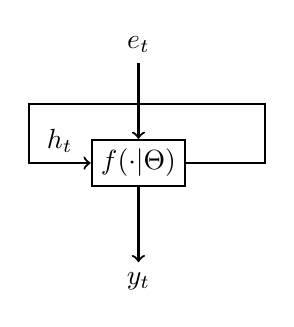
\begin{tikzpicture}[node distance=1.5cm, auto, thick]
        % Nodes
        \node (f) [draw, rectangle] {$f(\cdot|\Theta)$};
        \node (e) [above of=f] {$e_t$};
        \node (y) [below of=f] {$y_t$};

        % Edges
        \draw[->] (e) -- (f);
        \draw[->] (f) -- (y);
        \draw[->] (f.east) -- +(1,0) -- +(1,0.75) -- +(-2,0.75) -- +(-2,0) -- (f.west) node[above, pos=0.5] {$h_t$};
    \end{tikzpicture}
    \caption{RNN model}
    \label{fig:rnn_model}
\end{figure}



\subsection{Attention}
\label{sec:attention}

Imagine we have a dictionary:
\[
    D={(k_1,v_1),(k_2,v_2),\ldots,(k_m,v_m)}
\]
With $k_i\in\mathbb{R}^{k}$ and $v_i\in\mathbb{R}^{v}$.
Let's suppose this is a dictionary of vectors, where keys and values can be different dimensions.
Let's also assume that all keys are different. If this holds this is a vector dictionary.
The main problem that we have to solve on a dictionary is the \textbf{lookup}. We are given a \textbf{query}
in the same space of the keys.
The goal is to find $v_i$ if $k_i=q$ else return $0$.
In this case with vectors made of real numbers, if we were to implement it in this way it would be useless.
We relax the problem and change it to a soft lookup:
We check all the nearby keys and we return a weighted sum of the values of the nearby keys, the weight is 
computed with a sort of score function.

The contribution is calculated with a score function $a$:
\[
    a:\mathbb{R}^{k}\times\mathbb{R}^{k}\rightarrow\mathbb{R}
\]
that takes the query and the key and returns a scalar.

Because we run this function for the whole dictionary we will end up having
$m$ different values.
These numbers are called \textbf{attention scores}.
We want to select an $a$ that gives us \textbf{convex combinations} of the values.
To do this the sum of the scores must equal $1$.
We call this specific type of attention function $\alpha$.

We define the soft\_lookup operation as:
\[
    \text{soft\_lookup}(q,D)=\sum_{i=1}^{m}\alpha(q,k_i)v_i
\]

The attention is called like this because we compute how "important" the keys are for the query.

How do we compute the attention scores? We need to compute the similarity between the query and the keys,
to do this we use the \textbf{dot product}:
\[
    a(q,k_i)=q\cdot k_i
\]
Now we have to keep the sum of those scores equal to $1$, to do this we use the \textbf{softmax} function.
So the attention function is:
\[
    \alpha(q,k_i)=\left(\text{softmax}([a(q,k_1),a(q,k_2),\ldots,a(q,k_m)])\right)_i
\]
This is not the only way to compute attention but it's the simplest one.

We want to keep the variance under control, because a high variance can lead to numerical instability.
Assume that all components of the keys and queries are normally distributed ($N(0,1)$), let's see what happens to their dot product:
\[
    E[a(q,k_i)]=E[q\cdot k_i]=E\left[\sum_{j=1}^{k}q_jk_{ij}\right]=\sum_{j=1}^{k}E[q_j]E[k_{ij}]=0
\]
\[
    V[a(q,k_i)]=E[(q\cdot k_i)^2]-E[q\cdot k_i]^2=E[(q\cdot k_i)^2]
\]
Because the mean is $0$. Then:
\[
    E[(q\cdot k_i)^2]=E\left[(\sum_{j=1}^{k}q_jk_{ij})^2\right]=\sum_{j=1}^{k}E[q_j^2]E[k_{ij}^2]=k
\]
So the variance of the dot product is $k$.
At certain point during the backpropagation, the gradients explode. This happens because the variance of the dot product is not $1$.
The way to get variance 1 is to divide the dot product by $\sqrt{k}$:
\[
    a(q,k_i)=\frac{q\cdot k_i}{\sqrt{k}}
\]
The $\alpha$ function that we get is called \textbf{scaled dot product attention}.

We want to make this computation fast. To do this we want to make it as parallel as possible.

Remember that:
\begin{itemize}
    \item $q\in\mathbb{R}^{1\times k}$
    \item $m$ $k_i\in\mathbb{R}^{1\times k}$
    \item $m$ $v_i\in\mathbb{R}^{1\times v}$
\end{itemize}

We create a matrix $K$ with all the keys and a matrix $V$ with all the values:
\[
    K=\begin{bmatrix}
        k_1\\
        k_2\\
        \vdots\\
        k_m
    \end{bmatrix}
\]
\[
    V=\begin{bmatrix}
        v_1\\
        v_2\\
        \vdots\\
        v_m
    \end{bmatrix}
\]
And they are respectively of size $m\times k$ and $m\times v$.
We want to compute all the attention scores in parallel (we need to compute $qk_i^T$ for every $i$).
If we transpose $K$ we can compute all the scaled dot products in one go with $\frac{qK^T}{\sqrt{k}}$.
Then we apply the \textbf{softmax} function to get the all the attention scores $\alpha_i$ in a single vector.
Now we need to compute the combinations of the values, we can do this with a matrix multiplication:
\[
    \tilde{v}=[\alpha_1,\alpha_2,\ldots,\alpha_m]V
\]
$\tilde{v}$ is a vector of size $1\times v$.

Let's write it all together:
\[
    \tilde{v}=\text{softmax}\left(\frac{qK^T}{\sqrt{k}}\right)V
\]
This is called the \textbf{scaled dot attention} for a single query.

Now we want to compute it for $n$ queries, let's stack them in a matrix $Q$:
\[
    Q=\begin{bmatrix}
        q_1\\
        q_2\\
        \vdots\\
        q_n
    \end{bmatrix}
\]
$Q$ is of size $n\times k$.

Now what happens if we plug $Q$ into the formula?
We get $QK^T$ which is of size $n\times m$.
We can see that the elements of the matrix are the dot products of the queries with the keys.
\[
    QK^T=\begin{bmatrix}
        q_1k_1^T & q_1k_2^T & \ldots & q_1k_m^T\\
        q_2k_1^T & q_2k_2^T & \ldots & q_2k_m^T\\
        \vdots & \vdots & \ddots & \vdots\\
        q_nk_1^T & q_nk_2^T & \ldots & q_nk_m^T
    \end{bmatrix}
\]
We can apply the softmax function \textbf{at row level} to get:
\[
    \text{softmax}_\text{row}(\frac{QK^T}{\sqrt{k}})=\begin{bmatrix}
        \alpha_{11} & \alpha_{12} & \ldots & \alpha_{1m}\\
        \alpha_{21} & \alpha_{22} & \ldots & \alpha_{2m}\\
        \vdots & \vdots & \ddots & \vdots\\
        \alpha_{n1} & \alpha_{n2} & \ldots & \alpha_{nm}
    \end{bmatrix}
\]
That are the attention scores for all the queries.
By multiplying this matrix with $V$ we get:
\[
    \text{softmax}_\text{row}(\frac{QK^T}{\sqrt{k}})V=\begin{bmatrix}
        \tilde{v}_1\\
        \tilde{v}_2\\
        \vdots\\
        \tilde{v}_n
    \end{bmatrix}
\]
That are the values for all the queries.
The resulting formula is:
\[
    \tilde{V}=\text{softmax}_\text{row}\left(\frac{QK^T}{\sqrt{k}}\right)V
\]
This is the \textbf{scaled dot attention} for multiple queries.

What is the complexity of this operation?
Let's assume that $k=v=d$
The overall complexity is $O(nmd)$.
If the number of queries and keys is comparable and $d$ is much smaller than $m$
the complexity is $O(n^2)$. So the complexity is \textbf{quadratic}.

\subsection{Learnable Attention Mechanisms}
\label{sec:learnable-attention-mechanisms}

\subsubsection{Self-attention}

A way to use attention is called \textbf{self-attention}.
\[
    \tilde{X}=\text{softmax}_\text{row}(\frac{XX^T}{\sqrt{k}})X=\text{Attention}(X,X,X)=\text{SelfAttention}(X)
\]

We can see that:
\[
    XX^T=\begin{bmatrix}
    x_1x_1^T & x_1x_2^T & \ldots & x_1x_n^T\\
    x_2x_1^T & x_2x_2^T & \ldots & x_2x_n^T\\
    \vdots & \vdots & \ddots & \vdots\\
    x_nx_1^T & x_nx_2^T & \ldots & x_nx_n^T
    \end{bmatrix}
\]

So we are computing how much each word is similar to
every other word in the sentence.
We then use the softmaxed attention scores to compute the
weighted sum of the values (the same sentence).
So $\tilde{x}_1$ is going to be $\sum_{i=1}^{n}\alpha_ix_i$.
This process changes the embeddings for each word,
making it more appropriate for the context.

This process is still $O(n^2)$.

When we have a sentence that is generated with time,
at each time step we can "see" only the previous words.
How can we still parallelize this process if all the $X$ matrices
are different at each time step? (e.g. $X_1=[x_1], X_2=[x_1, x_2]$ etc.)
We want that each word computes its similarity only with 
previous words. How can we make the future words get an
attention score of $0$? We need to set the similarity to
$-\infty$ to make the softmax output $0$. To achieve this
we can set the upper triangular part of the matrix to $-\infty$.
Like this:
\[
    \frac{XX^T}{\sqrt{k}}+M=\begin{bmatrix}
        a_{11} && \ldots && a_{1n}\\
        \vdots && \ddots && \vdots\\
        a_{n1} && \ldots && a_{nn}
    \end{bmatrix} + \begin{bmatrix}
        0 & -\infty & \ldots & -\infty\\
        0 & 0 & \ldots & -\infty\\
        \vdots & \vdots & \ddots & \vdots\\
        0 & 0 & \ldots & 0
    \end{bmatrix}
\]

We call the matrix $M$ a \textbf{causal mask} and the operation is called \textbf{causal self-attention}.

\subsubsection{Attention head}

By default there's nothing that can learn in the attention mechanism.
Assume that we have a:
\begin{itemize}
    \item queries $Q$
    \item keys $K$
    \item values $V$
\end{itemize}
We can learn a projection for each of them.
So we compute:
\begin{itemize}
    \item $Q'=QW_Q$
    \item $K'=KW_K$
    \item $V'=VW_V$
\end{itemize}
Instead of computing the attention scores with $Q$ and $K$ we use $Q'$ and $K'$ and then
we use $V'$ to compute the weighted sum.
\[
    \tilde{V}=\text{softmax}_\text{row}(\frac{QW_q(KW_K)^T}{\sqrt{k}})VW_V
\]
Matrices $W_Q$, $W_K$ and $W_V$ do not need to be square, they can be of any size with the constraint
that $W_Q$ and $W_K$ go to the same output size.
\begin{figure}[H]
    \centering
    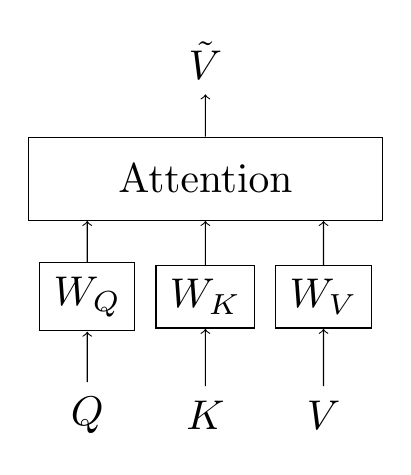
\begin{tikzpicture}[scale=1.5, every node/.style={scale=1.5}]
        % Nodes
        \node (K) {$K$};
        \node (Q) [left of=K] {$Q$};
        \node (V) [right of=K] {$V$};
        \node (W_K) [draw, rectangle, above of=K] {$W_K$};
        \node (W_Q) [draw, rectangle, above of=Q] {$W_Q$};
        \node (W_V) [draw, rectangle, above of=V] {$W_V$};
        \node (attention) [draw, rectangle, above of=W_K, minimum width=3cm, minimum height=0.7cm] {Attention};
        \node (output) [above of=attention] {$\tilde{V}$};

        % Arrows
        \draw [->] (Q) -- (W_Q);
        \draw [->] (K) -- (W_K);
        \draw [->] (V) -- (W_V);
        \draw [->] (W_Q) -- (W_Q.north |- attention.south);
        \draw [->] (W_K) -- (attention);
        \draw [->] (W_V) -- (W_V.north |- attention.south);
        \draw [->] (attention) -- (output);
    \end{tikzpicture}
    \caption{Attention Head}
    \label{fig:attention-head}
\end{figure}

This can be used as a layer in a neural network because it has learnable parameters.
The matrices $W_Q$, $W_K$ and $W_V$ learn how to project the queries, keys and values in compatible spaces.

\subsubsection{Multi-head attention}

Can we know if the learned projections are the best ones?
Of course not, but we can learn multiple different projections to be safe.

So instead of using a single attention head, we can use multiple attention heads.
Each of them is receiving the same input $Q,K,V$ and learns different projections.
So with $h$ heads we will have $h$ different outputs.
\[
    \tilde{V}=[\tilde{V}_1,\tilde{V}_2,\ldots,\tilde{V}_h]
\]
And then, with the concatenated output, we compute:
\[
    \tilde{\tilde{V}}=\tilde{V}W_O
\]
Where $W_O$ is a learnable matrix.

\begin{figure}[H]
    \centering
    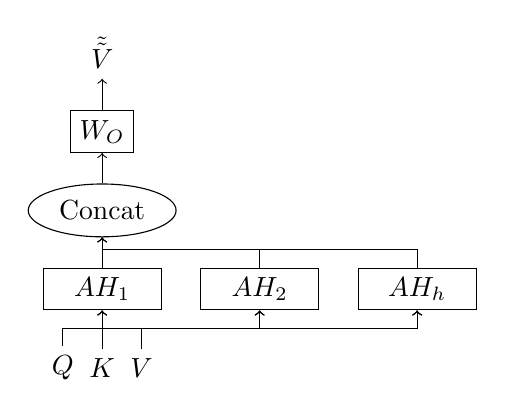
\begin{tikzpicture}
        % Nodes
        \node (K) {$K$};
        \node (Q) [left of=K, node distance=0.5cm] {$Q$};
        \node (V) [right of=K, node distance=0.5cm] {$V$};
        \node (AH_1) [draw, rectangle, above of=K, minimum width=1.5cm] {$AH_1$};
        \node (AH_2) [draw, rectangle, right of=AH_1, node distance=2cm, minimum width=1.5cm] {$AH_2$};
        \node (AH_h) [draw, rectangle, right of=AH_2, node distance=2cm, minimum width=1.5cm] {$AH_h$};
        \node (concat) [draw, ellipse, above of=AH_1] {Concat};
        \node (W_O) [draw, rectangle, above of=concat] {$W_O$};
        \node (output) [above of=W_O] {$\tilde{\tilde{V}}$};

        % Arrows
        \draw [->] (Q) |- ++(0,0.5) -| (AH_1);
        \draw [->] (K) |- ++(0,0.5) -| (AH_1);
        \draw [->] (V) |- ++(0,0.5) -| (AH_1);
        \draw [->] (Q) |- ++(0,0.5) -| (AH_2);
        \draw [->] (V) |- ++(0,0.5) -| (AH_2);
        \draw [->] (K) |- ++(0,0.5) -| (AH_2);
        \draw [->] (Q) |- ++(0,0.5) -| (AH_h);
        \draw [->] (K) |- ++(0,0.5) -| (AH_h);
        \draw [->] (V) |- ++(0,0.5) -| (AH_h);
        \draw [->] (AH_1) |- ++(0,0.5) -| (concat);
        \draw [->] (AH_2) |- ++(0,0.5) -| (concat);
        \draw [->] (AH_h) |- ++(0,0.5) -| (concat);
        \draw [->] (concat) -- (W_O);
        \draw [->] (W_O) -- (output);
    \end{tikzpicture}
    \caption{Multi Head Attention}
    \label{fig:multi-head-attention}
\end{figure}

We can summarize the multi-head attention as:
\[
    \tilde{\tilde{V}}=MHA(Q,K,V|W_I,W_O)
\]
Summarizing all the input transformations for each head with $W_I$ and the output transformation with $W_O$.
We can use self attention and/or causal self attention in the multi-head attention.

\subsubsection{Training MHA}

We want to avoid two things:
\begin{itemize}
    \item Overfitting
    \item "Burning" neurons (neurons don't learn anything)
\end{itemize}

To avoid burning neurons we want to make the variance under control (to avoid exploding/vanishing gradients).
We want to avoid that in a single input there is a lot of variance.
To do this we don't apply batch normalization, but we use \textbf{layer normalization}.

If the input is $x\in\mathbb{R}^{1\times k}$ and the output is $y\in\mathbb{R}^{1\times k}$, we compute the layer normalization as:
\[
    y=\frac{x-\mu_x}{\sigma_x}
\]
Where $\mu_x=1/k\sum_{i=1}^{k}x_i$ and $\sigma_x=\sqrt{1/k\sum_{i=1}^{k}(x_i-\mu_x)^2 + \epsilon}$.
With $\epsilon$ a small number to avoid division by zero.

We can let this layer learn by adding two learnable parameters $\alpha$ and $\beta$:
\[
    \text{LayerNorm}(x|\alpha,\beta)=\alpha\frac{x-\mu_x}{\sigma_x}+\beta
\]

The second mechanism to avoid burning neurons is the \textbf{skip/residual connection}.

\begin{figure}[H]
    \centering
    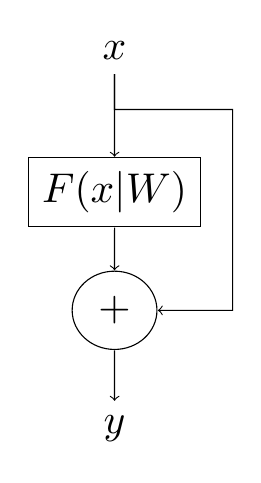
\begin{tikzpicture}[scale=1.5, every node/.style={scale=1.5}]
        % Nodes
        \node (input) {$x$};
        \node (layer) [draw, rectangle, below of=input, node distance=1.2cm] {$F(x|W)$};
        \node (sum) [draw, ellipse, below of=layer, node distance=1cm] {$+$};
        \node (output) [below of=sum, node distance=1cm] {$y$};

        % Arrows
        \draw [->] (input) -- (layer);
        \draw [->] (layer) -- (sum);
        \draw [->] (sum) -- (output);
        \draw [->] (input) -- ++(0,-0.5) -| ++(1,-1) |- (sum);
    \end{tikzpicture}
    \caption{Skip Connection}
    \label{fig:skip-connection}
\end{figure}

When using residual connections we risk having a huge variance in the earlier layers, to avoid this
we never use residual without a normalization mechanism like layer normalization.


\end{document}